\documentclass[a4paper,11pt,twoside]{report}


% -------------- Kodowanie znaków, język polski -------------

\usepackage[utf8]{inputenc}
\usepackage[MeX]{polski}
%\usepackage[T1]{fontenc}
\usepackage[english, polish]{babel}


% ----------------- Przydatne pakiety ----------------------
\usepackage{amsfonts}
\usepackage{mathrsfs} 
\usepackage{amsmath,amsthm,latexsym,xpatch}
\usepackage[dvips]{graphicx,color}
\usepackage{enumerate}
\usepackage{enumitem}
\usepackage{verbatim}
\usepackage{array}
\usepackage{pstricks}
\usepackage{textcomp}
\usepackage{listings}
\usepackage{xcolor}
\usepackage[none]{hyphenat}
\usepackage{float}
\usepackage{flafter}

% ---------------- Marginesy, akapity, interlinia ------------------

\usepackage[inner=20mm, outer=20mm, bindingoffset=10mm, top=25mm, bottom=25mm]{geometry}


\linespread{1.15}
%\allowdisplaybreaks
\usepackage{indentfirst} % opcjonalnie; pierwszy akapit z wcięciem
\setlength{\parindent}{5mm}

\hyphenation{Syl-ves-tra}
\hyphenation{Syl-ves-ter-a}

%--------------------------- ŻYWA PAGINA ------------------------

\usepackage{fancyhdr}
\pagestyle{fancy}
\fancyhf{}
% numery stron: lewa do lewego, prawa do prawego 
\fancyfoot[LE,RO]{\thepage} 
% prawa pagina: zawartość \rightmark do lewego, wewnętrznego (marginesu) 
\fancyhead[LO]{\sc \nouppercase{\rightmark}}
% lewa pagina: zawartość \leftmark do prawego, wewnętrznego (marginesu) 
\fancyhead[RE]{\sc \leftmark}

\renewcommand{\chaptermark}[1]{
\markboth{\thechapter.\ #1}{}}

% kreski oddzielające paginy (górną i dolną):
\renewcommand{\headrulewidth}{0 pt} % 0 - nie ma, 0.5 - jest linia


\fancypagestyle{plain}{% to definiuje wygląd pierwszej strony nowego rozdziału - obecnie tylko numeracja
  \fancyhf{}%
  \fancyfoot[LE,RO]{\thepage}%
  
  \renewcommand{\headrulewidth}{0pt}% Line at the header invisible
  \renewcommand{\footrulewidth}{0.0pt}
}



% ---------------- Nagłówki rozdziałów ---------------------

\usepackage{titlesec}
\titleformat{\chapter}%[display]
  {\normalfont\Large \bfseries}
  {\thechapter.}{1ex}{\Large}

\titleformat{\section}
  {\normalfont\large\bfseries}
  {\thesection.}{1ex}{}
\titlespacing{\section}{0pt}{30pt}{20pt} 
%\titlespacing{\co}{akapit}{ile przed}{ile po} 
    
\titleformat{\subsection}
  {\normalfont \bfseries}
  {\thesubsection.}{1ex}{}


% ----------------------- Spis treści ---------------------------
\def\cleardoublepage{\clearpage\if@twoside
\ifodd\c@page\else\hbox{}\thispagestyle{empty}\newpage
\if@twocolumn\hbox{}\newpage\fi\fi\fi}


% kropki dla chapterów
\usepackage{etoolbox}
\makeatletter
\patchcmd{\l@chapter}
  {\hfil}
  {\leaders\hbox{\normalfont$\m@th\mkern \@dotsep mu\hbox{.}\mkern \@dotsep mu$}\hfill}
  {}{}
\makeatother

\usepackage{titletoc}
\makeatletter
\titlecontents{chapter}% <section-type>
  [0pt]% <left>
  {}% <above-code>
  {\bfseries \thecontentslabel.\quad}% <numbered-entry-format>
  {\bfseries}% <numberless-entry-format>
  {\bfseries\leaders\hbox{\normalfont$\m@th\mkern \@dotsep mu\hbox{.}\mkern \@dotsep mu$}\hfill\contentspage}% <filler-page-format>

\titlecontents{section}
  [1em]
  {}
  {\thecontentslabel.\quad}
  {}
  {\leaders\hbox{\normalfont$\m@th\mkern \@dotsep mu\hbox{.}\mkern \@dotsep mu$}\hfill\contentspage}

\titlecontents{subsection}
  [2em]
  {}
  {\thecontentslabel.\quad}
  {}
  {\leaders\hbox{\normalfont$\m@th\mkern \@dotsep mu\hbox{.}\mkern \@dotsep mu$}\hfill\contentspage}
\makeatother



% ---------------------- Spisy tabel i obrazków ----------------------

\renewcommand*{\thetable}{\arabic{chapter}.\arabic{table}}
\renewcommand*{\thefigure}{\arabic{chapter}.\arabic{figure}}
%\let\c@table\c@figure % jeśli włączone, numeruje tabele i obrazki razem


% --------------------- Definicje, twierdzenia etc. ---------------


\makeatletter
\newtheoremstyle{definition}%    % Name
{3ex}%                          % Space above
{3ex}%                          % Space below
{\upshape}%                      % Body font
{}%                              % Indent amount
{\bfseries}%                     % Theorem head font
{.}%                             % Punctuation after theorem head
{.5em}%                            % Space after theorem head, ' ', or \newline
{\thmname{#1}\thmnumber{ #2}\thmnote{ (#3)}}%  % Theorem head spec (can be left empty, meaning `normal')
\makeatother

% ----------------------------- POLSKI --------------------------------
\theoremstyle{definition}
\newtheorem{theorem}{Twierdzenie}[chapter]
\newtheorem{lemma}[theorem]{Lemat}
\newtheorem{example}[theorem]{Przykład}
\newtheorem{proposition}[theorem]{Stwierdzenie}
\newtheorem{corollary}[theorem]{Wniosek}
\newtheorem{definition}[theorem]{Definicja}
\newtheorem{remark}[theorem]{Uwaga}

% If in English, comment this and uncomment below:

% ----------------------------- ENGLISH -----------------------------
%\theoremstyle{definition}
%\newtheorem{theorem}{Theorem}[chapter]
%\newtheorem{lemma}[theorem]{Lemma}
%\newtheorem{example}[theorem]{Example}
%\newtheorem{proposition}[theorem]{Proposition}
%\newtheorem{corollary}[theorem]{Corollary}
%\newtheorem{definition}[theorem]{Definition}
%\newtheorem{remark}[theorem]{Remark}



% ----------------------------- Dowód -----------------------------

\makeatletter
\renewenvironment{proof}[1][\proofname]
{\par
  \vspace{-12pt}% remove the space after the theorem
  \pushQED{\qed}%
  \normalfont
  \topsep0pt \partopsep0pt % no space before
  \trivlist
  \item[\hskip\labelsep
        \sc
    #1\@addpunct{:}]\ignorespaces
}
{%
  \popQED\endtrivlist\@endpefalse
  \addvspace{20pt} % some space after
}

\renewcommand{\qedhere}{\hfill \qedsymbol}
\makeatother





% -------------------------- POCZĄTEK --------------------------


% --------------------- Ustawienia użytkownika ------------------

\newcommand{\tytul}{Gogle AR jako modyfikacja gogli VR}
\renewcommand{\title}{AR googles as modified VR googles}
\renewcommand{\author}{Dawid Łazuk, Piotr Piwowarski}
\newcommand{\album}{268791,000000}
\newcommand{\type}{inżyniers} % magisters, licencjac (Master or Engineer in English)
\newcommand{\supervisor}{dr inż. Krzysztof Kaczmarski}

\lstdefinestyle{sharpc}{language=[Sharp]C, rulecolor=\color{blue!80!black}}

\begin{document}
\sloppy

% \selectlanguage{english} % uncomment this for English 

% ----------------------- Abstrakty -----------------------------

%\selectlanguage{polish}
\begin{abstract}

\begin{center}
\tytul
\end{center}

Lorem ipsum dolor sit amet, consetetur sadipscing elitr, sed diam nonumyeirmod tempor invidunt ut labore et dolore magna aliquyam erat, sed diamvoluptua. At vero eos et accusam et justo duo dolores et ea rebum. Stet clita kasd gubergren, no sea takimata sanctus est Lorem ipsum dolor sit amet.\\

\noindent \textbf{Słowa kluczowe:} slowo1, slowo2, ...
\end{abstract}

\null\thispagestyle{empty}\newpage

{\selectlanguage{english}
\begin{abstract}

\begin{center}
\title
\end{center}

Lorem ipsum dolor sit amet, consetetur sadipscing elitr, sed diam nonumyeirmod tempor invidunt ut labore et dolore magna aliquyam erat, sed diamvoluptua. At vero eos et accusam et justo duo dolores et ea rebum. Stet clita kasd gubergren, no sea takimata sanctus est Lorem ipsum dolor sit amet.

Lorem ipsum dolor sit amet, consetetur sadipscing elitr, sed diam nonumyeirmod tempor invidunt ut labore et dolore magna aliquyam erat, sed diamvoluptua. At vero eos et accusam et justo duo dolores et ea rebum. Stet clita kasd gubergren, no sea takimata sanctus est Lorem ipsum dolor sit amet.\\

\noindent \textbf{Keywords:} keyword1, keyword2, ...
\end{abstract}}


\null\thispagestyle{empty}\newpage

\null \hfill Warszawa, dnia ..................\\

\par\vspace{5cm}

\begin{center}
Oświadczenie % Declaration - for English
\end{center}

\indent Oświadczam, że pracę \type ką pod
tytułem ,,\tytul '', której promotorem jest \supervisor \ wykonałam/em
samodzielnie, co poświadczam własnoręcznym podpisem.
\vspace{2cm}

% English:

%I hereby declare that the thesis entitled ,,\title '', submitted for the \type ~degree, supervised  by \supervisor , is entirely my original work apart from the recognized reference.
%\vspace{2cm}

\begin{flushright}
  \begin{minipage}{50mm}
    \begin{center}
      ..............................................

    \end{center}
  \end{minipage}
\end{flushright}

\thispagestyle{empty}
\newpage

\null\thispagestyle{empty}\newpage
% ------------------- 4. Spis treści ---------------------
% \selectlanguage{english} - for English

\tableofcontents
\thispagestyle{empty}
\newpage
% -------------- 5. ZASADNICZA CZĘŚĆ PRACY --------------------
\null\thispagestyle{empty}\newpage
\setcounter{page}{11}
\pagestyle{fancy}


\chapter*{Wstęp} % Intruduction
\markboth{}{Wstęp}
\addcontentsline{toc}{chapter}{Wstęp}

Szybki rozwój techniki spowodował zwiększenie jej obecności w codziennym życiu. Rozwój interfejsów użytkownika i badania nad jego wrażeniami z wykorzystywania różnych systemów spowodowały powstanie technologii takich jak wirtualna rzeczywistość i rozszerzona rzeczywistość. Służą one zarówno do rozrywki jak i też do ułatwienia życia i usprawnienia pracy ludziom. Rozwiązania tego typu stają się coraz popularniejsze i można zaobserwować rosnące nimi zainteresowanie w wielu branżach.

Dlatego też, w niniejszej pracy podjęto się zbadania możliwości zastosowania gogli wirtualnej rzeczywistości w aplikacjach wykorzystujących rzeczywistość rozszerzoną. Stworzony zostanie system, który umożliwia przekazanie obrazu widzianego przez kamery, symulujące ludzkie oczy, do gogli wirtualnej rzeczywistości. Powstałe w ten sposób ``wirtualne okulary'' będą mogły zostać wykorzystane do uruchomienia na nich aplikacji przeznaczonych na systemy rozszerzonej rzeczywistości.

Po stworzeniu tego systemu, zbadano czy wizja uzyskana z wykorzystaniem gogli wirtualnej rzeczywistości połączonych z kamerami znacznie różni się od naturalnej wizji człowieka i jeżeli tak, to jak to wpływa na komfort i możliwość korzystania z systemu. Opisano związane z tym problemy oraz dalsze kroki, jakie należy podjąć tworząc tego typu rozwiązania.

\chapter{Technologia VR/AR. Zmysł wzroku.}

W tym rozdziale omówione zostaną zagadnienia wirtualnej oraz rozszerzonej rzeczywistości. Poruszone zostaną problemy, jakie wiążą się z zastosowaniem tych technologii. Przedstawiona zostanie też natura widzenia stereoskopowego człowieka w zakresie zjawisk, które będą miały wpływ na przebieg prac i ich rezultat.

\section{Wirtualna i rozszerzona rzeczywistość}

\subsection{Definicje i zastosowanie VR/AR}

\begin{definition}[Wirtualna rzeczywistość]
\textit{Wirtualną rzeczywistością} (ang. VR - Virtual Reality) nazywamy wrażenie przebywania użytkownika w świecie stworzonym wirtualnie. Zwykle dotyczy to obrazu, dźwięku oraz interakcji z otoczeniem, ale podejmowane są próby wykorzystania zapachu i dotyku w aplikacjach VR.
\end{definition}

Obecnie większości ludziom termin VR kojarzy się z goglami zakładanymi na głowę użytkownika, które umożliwiają wyświetlanie sceny 3D w taki sposób, że użytkownik ma wrażenie przebywania w tej scenie. Wbudowane w urządzenie żyroskopy reagują na ruchy głowy odwzorowując je w wyświetlanym obrazie. Gogle często posiadają wbudowane głośniki (Oculus Rift) lub możliwość podpięcia słuchawek (HTC Vive), zapewniając także bodźce akustyczne. Takie rozwiązanie pozwala osiągnąć immersję nieosiągalną dla dotychczasowo wykorzystywanych technologii, nawet takich jak telewizja trójwymiarowa.

Wirtualna rzeczywistość jest obecnie stosowana na bardzo szeroką skalę. Wykorzystywana jest w przemyśle rozrywkowym w postaci gier VR czy też filmów 360\textdegree, w których użytkownik może poczuć się jakby znajdował się w samym centrum akcji. Rozwiązania VR mają potencjał w przemyśle turystycznym, umożliwiając wirtualne wycieczki po egzotycznych, często trudno dostępnych miejscach. Agenci nieruchomości mogą umożliwić zainteresowanym klientom obejrzenie mieszkania czy domu jeszcze przed powstaniem budynku. Wystarczy tylko stworzyć odpowiedni model 3D i wyświetlić go w goglach wirtualnej rzeczywistości. Technologia znalazła też zastosowanie w szkoleniu żołnierzy, umożliwiając przeprowadzenie symulacji operacji na~wirtualnych poligonach.\cite{VRdefinition}

\begin{definition}[Rozszerzona rzeczywistość]
\textit{Rozszerzoną rzeczywistością} (ang. AR - Augmented Reality) nazywamy nałożenie na wizję świata rzeczywistego obrazu stworzonego wirtualnie. Użytkownik dzięki temu może na przykład otrzymywać dodatkowe informacje o~obiektach, na które patrzy.
\end{definition}

Rozwiązania rozszerzonej rzeczywistości wzbogacają zmysły człowieka poprzez przekazanie im dodatkowych informacji. O ile w przypadku wirtualnej rzeczywistości użytkownik, w pewnym sensie, odcinał się od świata rzeczywistego, tak w przypadku rzeczywistości rozszerzonej ten kontakt z rzeczywistością pozostaje. Istnieją samochody oraz myśliwce wyposażone w HUD - przezroczysty ekran wyświetlający informacje takie jak na przykład prędkość, z jaką porusza się samochód, nie zasłaniając tego co za nim się znajduje. Dość znanym zastosowaniem rozszerzonej rzeczywistości jest, wydana w 2016 roku, gra Pokemon GO. Użytkownik przy pomocy swojego smartphone'a spacerując po mieście zbiera pokemony, które wyświetlają się na ekranie telefonu jako obraz nałożony na  świat rzeczywisty, widziany przez kamerę urządzenia.

Przykładami urządzeń AR obecnymi na rynku są Google Glass i Microsoft HoloLens. W odróżnieniu od wirtualnej rzeczywistości, oczy użytkownika nie zostają zasłonięte całkowicie. Urządzenia mają formę okularów, przez które człowiek widzi to co przed nim się znajduje, a~obraz wirtualny jest wyświetlany na okularach bądź aplikowany bezpośrednio do oka.

\begin{definition}[Mieszana rzeczywistość]
\textit{Mieszaną rzeczywistością} (ang. MR - Mixed Reality) nazywamy rozszerzenie klasy rozwiązań AR o interakcję użytkownika z wirtualną częścią świata.
\end{definition}

Niektóre źródła\cite{ARMRdifferences} rozróżniają rozszerzoną rzeczywistość od mieszanej rzeczywistości utrzymując, że rozwiązania AR nie zapewniają interakcji z wirtualną częścią rzeczywistości. W związku z rozróżnieniem tych dwóch zagadnień, definicja mieszanej rzeczywistości została zamieszczona w niniejszej pracy. Zagadnienie to leży jednak poza jej zakresem, dlatego nie jest szerzej opisane. 

\subsection{Problemy użytkowe VR/AR}

Wykorzystanie rozwiązań wirtualnej i rozszerzonej rzeczywistości niesie za sobą szereg wyzwań stawianych deweloperom, oraz konsekwencji, których użytkownicy muszą być świadomi. W tym podrozdziale omówione zostały problemy, z jakimi wiąże się wykorzystanie VR/AR\cite{VRdifficulties}.

\begin{description}
\item [Wymogi wydajnościowe] \hfill \\
W celu komfortowego korzystania z rozwiązań wirtualnej rzeczywistości, systemy muszą spełniać szereg wymogów wydajnościowych. Organizm ludzki najlepiej akceptuje obraz o~częstotliwości zgodnej z częstotliwością pracy oka. Podanie obrazu o częstotliwości dużo niższej będzie powodowało dyskomfort w korzystaniu z aplikacji. Przyjmuje się, że obraz w aplikacjach VR powinien mieć conajmniej 60 FPS, aby zachować płynność obrazu. Jednak według wielu źródeł, do w pełni komfortowego korzystania z gogli konieczne jest osiągnięcie nawet 90 FPS\cite{VRframesPerSecond}. Opóźnienie obrazu powinno wynosić maksymalnie 15 ms\cite{VRlatency}, w celu uniknięcia niespójności pomiędzy np. wykonaniem ruchu głowy, którego mózg jest świadomy, a obrazem.
\item [Wpływ na wzrok] \hfill \\
Nie podlega wątpliwościom, że długotrwała praca przy monitorze szkodzi. Mięśnie gałki ocznej, które w normalnych warunkach są odpowiedzialne za akomodację oka, zastygają w jednej pozycji, ponieważ ekran jest w mniej więcej stałej odległości od oka. Intensywne światło też ma negatywny wpływ na oczy. W przypadku gogli wirtualnej rzeczywistości mamy do czynienia z relatywnie dużym ekranem, zasłaniającym praktycznie całe pole widzenia użytkownika, w odległości rzędu kilkudziesięciu milimetrów od oka. Długotrwała praca oczu w takich warunkach może doprowadzić do pogorszenia wzroku.
\item [Choroba symulacyjna] \hfill \\
Ludzki organizm jest skonstruowany tak, że mózg pobiera informacje dotyczące otoczenia z różnych zmysłów. W normalnych warunkach bodźce z różnych układów odbierane w tym samym czasie odpowiadają sobie. W zagadnieniach wirtualnej rzeczywistości układem zmysłów, powodującym problemy, jest układ oczy - błędnik. W grach lub filmach, w których występuje ruch, oczy użytkownika odbierają bodźce wskazujące na ruch organizmu. Natomiast jeśli użytkownik siedzi na przykład w fotelu, jego błędnik nie wykrywa ruchu. Mózg otrzymuje sprzeczne bodźce, co skutkuje objawami podobnymi do choroby lokomocyjnej, mimo braku jakiegokolwiek ruchu.\cite{VRsickness}
\item [Zbyt wysoka immersja] \hfill \\
Znane są przypadki ludzi umierających przed ekranem monitora po kilkunastu lub kilkudziesięciu godzinach nieustannej gry. Osoby uzależnione w takim stopniu od wirtualnej rozgrywki mają problem z rozróżnianiem świata rzeczywistego od wirtualnego, zapominając nawet o potrzebach fizjologicznych. Wysoka immersja, osiągana przez rozwiązania wirtualnej rzeczywistości, może spotęgować ten problem. Zwłaszcza, że rozrywka VR jest znacznie bardziej wymagająca dla organizmu od tradycyjnej, co już zostało wcześniej opisane. 
Kolejny problem dotyczący immersji jest związany z osobami mającymi problemy kardiologiczne. Realistyczne wrażenia z gier typu horror mogą doprowadzić takie osoby nawet do zawału serca.
\end{description}

\section{Wizja stereoskopowa człowieka}

Człowiek doświadcza widzenia trójwymiarowego dzięki temu, że dwoje jego oczu jest skierowane prawie równolegle w ten sam punkt. Umożliwia to zebranie dwóch podobnych do siebie obrazów. Różnica między nimi polega na przesunięciu oczu (kamer) względem siebie, przez co każdy obiekt jest widziany na jednym obrazie z nieco innej perspektywy, niż na drugim. Mózg nakładając na siebie te obrazy, dzięki tej różnicy, tworzy efekt głębi umożliwiając człowiekowi ocenę odległości przedmiotów, na które patrzy.

\subsection{Odległość między źrenicami}

Badania antropometryczne personelu armii Stanów Zjednoczonych w 2012 roku\cite{IPdistance} objęły swoim zakresem odległości między ludzkimi źrenicami. Wyniki tych badań są zawarte w poniższej tabeli. Dane są przedstawione w milimetrach.

\begin{table}[h!]
\centering
\label{my-label}
\begin{tabular}{lcccc}
\textbf{Płeć} & \multicolumn{1}{l}{\textbf{Minimum}} & \multicolumn{1}{l}{\textbf{Maksimum}} & \multicolumn{1}{l}{\textbf{Średnia}} & \multicolumn{1}{l}{\textbf{Mediana}} \\
Kobieta       & 51.0                                 & 74.5                                  & 61.7                                 & 62.0                                 \\
Mężczyzna     & 53.0                                 & 77.0                                  & 64.0                                 & 64.0                                
\end{tabular}
\caption{Odległości między źrenicami}
\end{table}

Z powyższych danych jednoznacznie wynika, że odległość pomiędzy ludzkimi źrenicami zawiera się w przedziale od 51.0 milimetrów do 77.0 milimetrów.

\subsection{Akomodacja oka}

\begin{definition}[Akomodacja oka]
\textit{Akomodacją oka} nazywamy zjawisko dostosowania się soczewki oka do odległości od oglądanego przedmiotu, w celu zapewnienia ostrości obrazu.
\end{definition}

U człowieka akomodacja oka jest realizowana poprzez zmianę kształtu soczewki, co skutkuje zmianą jej ogniskowej (zdolności skupiającej) \cite{eyeAccomodation}.

\begin{definition}[Punkt bliży wzrokowej]
\textit{Punktem bliży wzrokowej} nazywamy minimalną odległość, przy której akomodacja oka wpływa na ostrość obrazu. U człowieka punkt bliży wzrokowej leży w odległości $10 cm$ od oka.
\end{definition}

\begin{definition}[Punkt dali wzrokowej]
\textit{Punktem dali wzrokowej} nazywamy maksymalną odległość, przy której akomodacja oka wpływa na ostrość obrazu. U człowieka punkt dali wzrokowej leży w odległości $6 m$ od oka.
\end{definition}

\subsection{Zbieżność oczu}

\begin{definition}[Zbieżność oczu]
\textit{Zbieżnością oczu} nazywamy zjawisko obrócenia oczu do środka w sytuacji, kiedy obserwowany punkt leży w niewielkiej odległości od obserwatora. W~takim przypadku osie widzenia obu oczu przecinają się w jednym punkcie. Jeżeli natomiast obserwowany punkt leży daleko od obserwatora, osie widzenia są równoległe do siebie.\cite{eyeConvergence}
\end{definition}

\begin{figure}[h]
\centering
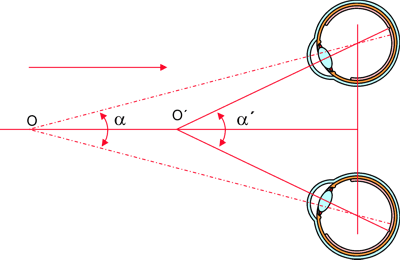
\includegraphics[scale=1]{images/zbieznosc}
\caption[Zbieżność oczu\cite{zbieznosc}]{Zbieżność oczu}
\end{figure}

\chapter{Cel i założenia projektu} % Cel i założenia projektu

Rozdział poświęcony jest opisaniu celu projektu, który powstał w ramach niniejszej pracy inżynierskiej. Wyspecyfikowane zostaną wymagania, jakie tworzony system musi spełniać.

\section{Funkcjonalność systemu}
System ma umożliwiać przekazanie obrazu z dwóch kamer do gogli wirtualnej rzeczywistości, tworząc tym samym gogle rozszerzonej rzeczywistości. Takie gogle następnie będą mogły posłużyć do wykorzystywania aplikacji przeznaczonych na rozwiązania AR. 

System ma umożliwiać efekt widzenia stereoskopowego, aby użytkownik miał wrażenie wizji zbliżonej do naturalnej, trójwymiarowej wizji człowieka. Efekt ten zostanie osiągnięty poprzez umiejscowienie kamer tak, aby odległość między ich soczewkami odpowiadała odległości pomiędzy źrenicami ludzkich oczu. 

System ma umożliwiać przetwarzanie przechwyconego obrazu zanim trafi on do oczu. Przetwarzanie to może być realizowane, na przykład, poprzez nałożenie prostych filtrów na obraz, lub też wykorzystania bardziej zaawansowanych algorytmów (na przykład wykrywania twarzy).

\section{Środowisko sprzętowe}
W tym podrozdziale omówione zostaną urządzenia wykorzystane w pracy. Przedstawiona zostanie specyfikacja sprzętu zapewnionego przez Wydział Matematyki i Nauk Informacyjnych Politechniki Warszawskiej. Omówimy także problemy wynikające z wykorzystania danego rodzaju sprzętu oraz propozycje ich rozwiązania.

\subsection{Gogle Oculus Rift}
Oculus Rift to gogle wirtualnej rzeczywistości stworzone przez firmę Oculus VR, będącą obecnie własnością Facebook Inc. Zostały ujawnione światu w 2012 roku na platformie Kickstarter w celu zebrania funduszy na rozwój projektu. 

Oculus Rift wykorzystuje dwa ekrany OLED, po jednym na każde oko. Ekrany te mają rozdzielczość 1080 pikseli na 1200 pikseli. Częstotliwość ich odświeżania wynosi 90 Hz. Pomiędzy ekranami, a oczami użytkownika znajdują się soczewki. Kąty widzenia gogli to 90\textdegree  pionowo i~80\textdegree  poziomo.

Gogle zostaną wykorzystane do wyświetlania obrazu przechwyconego przez kamery.

\subsection{Logitech Webcam C910 Pro HD}
C910 Pro HD to kamera USB stworzona przez firmę Logitech. Umożliwia przechwytywanie obrazu o rozdzielczości 1920 pikseli na 1080 pikseli. Posiada wbudowany mikrofon, jednak nie będzie on wykorzystywany w naszej pracy.

Wydział MiNI zapewnił dwa egzemplarze tych kamer na rzecz niniejszej pracy. W związku z tym, że panoramiczny obraz, standardowo zapewniany przez kamery, jest daleki od natury ludzkiego oka ograniczymy się do obrazu 4:3. Zatem rozdzielczość obrazu w naszej pracy będzie wynosiła 1440 pikseli na 1080 pikseli na jedno oko.

Obudowa tej kamery jest zbyt duża, szczególnie w pozycji poziomej. Jest to problemem, ponieważ minimalna odległość między soczewkami, na jaką możemy umieścić kamery w tej pozycji, wynosi około 100 milimetrów. Jest to znacznie powyżej górnego ograniczenia odległości między ludzkimi źrenicami. W związku z tym konieczne będzie umieszczenie tych kamer w~pozycji pionowej. Skutkuje to tym, że efektywna rozdzielczość przechwytywanego obrazu będzie wynosiła 1080 pikseli na 1440 pikseli.

\section{Odwzorowanie widzenia stereoskopowego}

Uzyskanie efektu widzenia trójwymiarowego, podczas używania gogli z zaimplementowanym rozwiązaniem, jest jednym z najważniejszych celów tego projektu. W tym podrozdziale znajduje się odniesienie do cech widzenia stereoskopowego, opisanych w poprzednim rozdziale, pod kątem tego, jak wpływają na tworzone rozwiązanie w ramach niniejszej pracy. 

\subsection{Parametryzacja widzenia}
Widzenie stereoskopowe można opisać trzema parametrami:
\begin{itemize}
\item Kąt widzenia kamer
\item Odległość między obiektywami kamer
\item Kąt odchylenia osi widzenia
\end{itemize}

Pierwszy z tych parametrów - kąt widzenia kamer, jest zależny bezpośrednio od modelu kamery zastosowanego w projekcie. Jedyna możliwa jego regulacja polega na obcięciu brzegów obrazu, zmniejszając tym samym kąt widzenia. W niniejszej pracy istotnym jest, aby kąt widzenia kamer był zbliżony do kąta widzenia zapewnianego przez gogle Oculus Rift.

Dwa kolejne - odległość między kamerami i odchylenie osi widzenia, są istotne przy uzyskaniu efektu głębi podczas patrzenia przez gogle. Przy założeniu, że obserwujemy jeden punkt, istnieje korelacja między tymi parametrami pozwalająca uzyskać efekt głębi patrząc na przedmioty w okolicy obserwowanego punktu nawet w sytuacji, gdy odległość, bądź odchylenie odbiegają od idealnego ustawienia dla danego użytkownika. Przykładem będzie odchylenie osi widzenia do środka w przypadku, gdy odległości między obiektywami są większe, niż między oczami użytkownika. Jednakże efekt w ten sposób uzyskany jest tylko punktowy, a obiekty położone w~innej odległości od punktu odniesienia nie będą widziane jako trójwymiarowe.

\subsection{Cechy zmysłu wzroku w projekcie}

W podrozdziale \textit{Widzenie stereoskopowe człowieka} zostały przedstawione cechy ludzkiego zmysłu wzroku, które mają wpływ na przebieg niniejszej pracy. W tym podrozdziale omówione zostaną założenia, jakie zostały podjęte podczas realizacji projektu w celu spełnienia tych wymagań, oraz uzasadnienie w przypadku braku możliwości spełnienia danego wymagania.

\begin{description}

\item[Odległość między źrenicami] \hfill \\
W celu zapewnienia komfortowego korzystania z systemu jak największej grupie użytkowników konieczne jest opracowanie sposobu umieszczenia kamer zapewniającego:
\begin{itemize}
\item Umieszczenie kamer w stałej odległości od siebie podczas użytkowania systemu
\item Regulację odległości kamer od siebie
\end{itemize}

Kamery docelowo miały zostać umieszczone na goglach, ale przewidziana jest możliwość mocowania ich na czym innym, jednak z zachowaniem punktów wymienionych powyżej.

\item [Akomodacja oka] \hfill \\
Zjawisko akomodacji oka w niniejszej pracy jest nie do odwzorowania z wykorzystaniem dostępnego sprzętu. Wymaga ono śledzenia gałki ocznej w celu wyznaczenia punktu, który jest obserwowany przez użytkownika, a następnie wyostrzenie obrazu w danym punkcie. Gogle Oculus Rift nie mają obecnie takiej możliwości.

\item[Zbieżność oczu] \hfill \\
Zjawisko zbieżności oczu w niniejszej pracy również jest nie do odwzorowania z takich samych powodów co zjawisko \textit{akomodacji oka}. Należałoby wyznaczyć punkt obserwowany przez użytkownika, a następnie skierować kamery w dany punkt. Wymagałoby to też stworzenia urządzenia, które poruszałoby kamerami w zależności od obserwowanego punktu. Wykracza to znacznie poza zakres realizowanej pracy.

\end{description}

\chapter{Implementacja projektu}
W tym rozdziale przedstawione zostaną efekty pracy. Omówione zostaną decyzje architektoniczne oraz szczegóły techniczne zaimplementowanego rozwiązania.

\section{Schemat systemu}

\subsection{Droga obrazu}
Planując wykonanie projektu droga, jaką musi przebyć obraz od przechwycenia go przez kamery do przekazania go do oka użytkownika, została podzielona na trzy warstwy. Są to:

\begin{description}
\item [Warstwa przechwytywania obrazu] \hfill \\ Jest odpowiedzialna za pobieranie obrazów z kamer i przygotowanie ich do dalszego przetwarzania - rotację obrazu w zależności od położenia kamery.
\item [Warstwa przetwarzania obrazu] \hfill \\ Wykonuje przetwarzanie obrazu według algorytmów zdefiniowanych przez użytkownika lub programistę.
\item [Warstwa przekazywania obrazu do gogli] \hfill \\ Odpowiada za konwersję obrazu do postaci przyjmowanej przez gogle VR.
\end{description}

\subsection{Architektura systemu}
System składa się z modułów realizujących ściśle określone zadania, dlatego też łatwo wydzielić je do osobnych projektów. Poniższy schemat przedstawia architekturę rozwiązania wraz z zaznaczonym kierunkiem przekazywania obrazu pomiędzy warstwami. 

\begin{figure}[h]
\centering
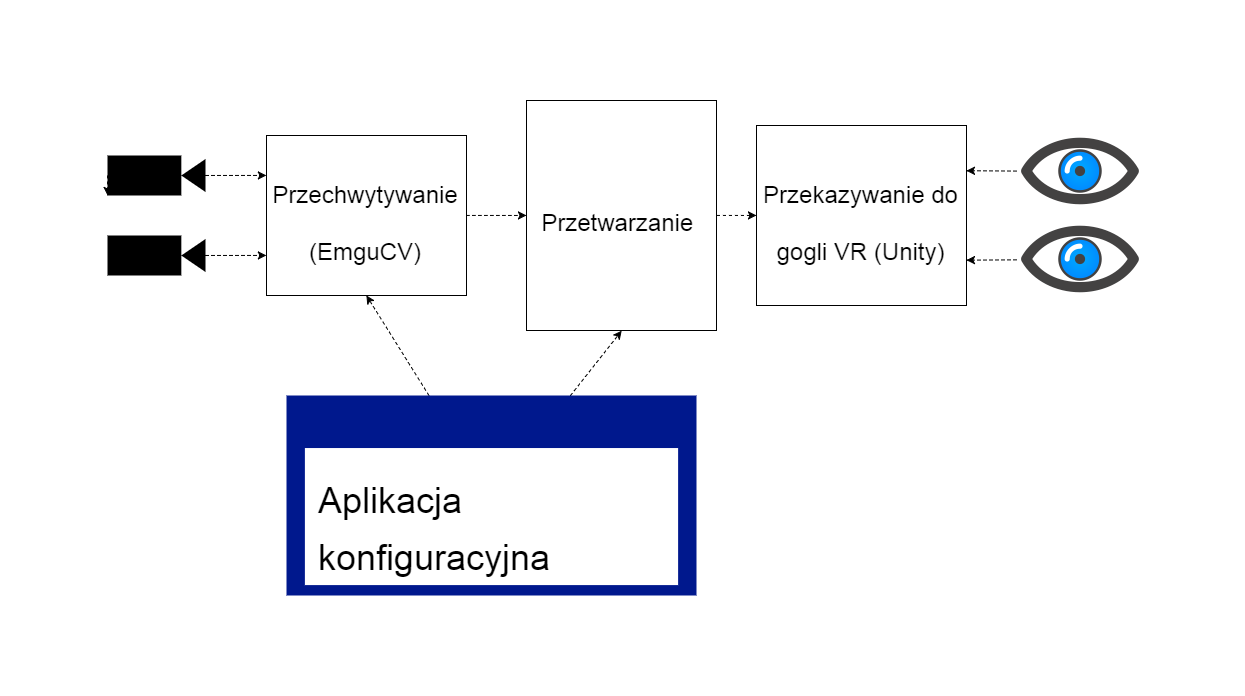
\includegraphics[scale=0.3]{images/architecture_schema}
\caption[Architektura systemu]{Architektura systemu}
\end{figure}

Jak widać na rysunku, obraz zanim trafi do oka przechodzi przez wszystkie warstwy. Najpierw przy użyciu biblioteki EmguCV obraz jest pobierany z kamer. Następnie przy użyciu stworzonych na potrzeby systemu klas, stosowane są dla niego odpowiednie przekształcenia. Końcowy efekt osiągany jest poprzez przesłanie przetworzonego obrazu do gogli VR, za pomocą aplikacji działającej przy użyciu silnika Unity. Aplikacja konfiguracyjna, która została stworzona z wykorzystaniem technologii WPF ,umożliwia modyfikację parametrów w warstwach przechwytywania i przetwarzania obrazu, podczas działania systemu. 

W celu zapewnienia podstawowego działania systemu, niezbędne są warstwy przechwytywania obrazu z kamer oraz przekazywania go do gogli. Warstwa przetwarzania obrazu jest opcjonalna i mogłaby być usunięta, lub chwilowo wyłączona z systemu, bez utraty jego podstawowych funkcjonalności. Równolegle do pozostałych warstw (nie bierze bezpośredniego udziału w drodze obrazu od kamer do oczu) działa  aplikacja konfiguracyjna, która zapewnia graficzny interfejs do sterowania działaniem systemu. Aplikacja działa w osobnym procesie, komunikując się z~głównym procesem wykorzystując serwis WCF.

\subsection{Funkcjonalność przetwarzania obrazu}
Funkcjonalność ta realizowana jest poprzez zastosowanie serii przekształceń do obrazu, podczas jego drogi do oczu użytkownika. System przewiduje możliwość dodawania nowych przekształceń. Obiekty, realizujące te przekształcenia muszą być utworzone według kontraktu, zdefiniowanego w dostarczonej bibliotece programistycznej. Przekształcenia wykonywane są w~ustalonej kolejności. Z poziomu aplikacji konfiguracyjnej możliwe jest zarządzenie kolejnością ich wykonywania lub wyłączenie części z nich.

\section{Wybrane technologie i oprogramowanie}
\subsection{Języki i technologie }
\begin{description}
\item [Język programowania C\# ] \hfill \\
System został wykonany z wykorzystaniem języka programowania C\# oraz platformy programistycznej .NET Framework. Wybór tej technologii był podyktowany doświadczeniem zespołu w jej wykorzystaniu. Również wykorzystany silnik Unity3D wspiera .NET co sugerowało uniknięcie przyszłych problemów integracją modułów. W~pracy .NET Framework został wykorzystany do napisania funkcjonalności pobierania obrazu z kamer i przetwarzania go, zanim trafi do modułu przekazywania obrazu do gogli.

\item [EmguCV] \hfill \\
Biblioteka opakowująca popularną bibliotekę do przetwarzania obrazów - OpenCV, w interfejs umożliwiający wykorzystanie jej w aplikacjach napisanych w języku C\#. Wykorzystana do implementacji modułów przechwytywania i przetwarzania obrazu. Przykładowe algorytmy przetwarzania obrazu również zostały napisane z wykorzystaniem tej biblioteki. 

\item [Silnik Unity3D] \hfill \\
Zintegrowane środowisko do tworzenia trójwymiarowych gier i innych materiałów interaktywnych.  Pozwala tworzyć aplikacje na przeglądarki internetowe, komputery osobiste, konsole gier wideo oraz urządzenia mobilne. Środowisko to zostało wybrane ze względu na łatwą integrację z pozostałymi używanymi technologiami. Zostało wykorzystane do stworzenia warstwy przekazywania obrazu do gogli Oculus Rift.

\item [Windows Presentation Foundation] \hfill \\
Windows Presentation Foundation (WPF) jest technologią służącą do tworzenia interfejsów użytkownika w aplikacjach desktopowych w środowisku .NET. W niniejszej pracy technologia ta została wykorzystana do napisania aplikacji konfiguracyjnej, która szerzej opisana będzie w dalszej części pracy.

\item [Windows Communication Foundation] \hfill \\
Windows Communication Foundation (WCF) jest technologią integrującą i unifikującą wszystkie technologie służące do komunikacji międzyprocesowej w aplikacjach opartych o~.NET Framework. W niniejszej pracy WCF został wykorzystany do zaimplementowania komunikacji pomiędzy procesem głównym systemu, a aplikacją konfiguracyjną.
\end{description}

Wszystkie wymienione technologie zostały wybrane do realizacji pracy, ponieważ zespół, który nad nią pracował, miał doświadczenie w pracy z nimi wyniesione z poprzednich projektów realizowanych w ramach studiów i pracy zawodowej.

\subsection{Oprogramowanie}
\begin{description}
\item [Microsoft Visual Studio] \hfill \\
Zintegrowane środowisko programistyczne firmy Microsoft. Jest to najpopularniejsze IDE wykorzystywane w tworzeniu aplikacji opartych o .NET Framework.
\item [SoapUI] \hfill \\
Aplikacja służąca do testów serwisów webowych. Wykorzystana przez nas do testów połączenia pomiędzy procesem głównym, a aplikacją konfiguracyjną.
\end{description}

\section{Opis modułów}

\subsection{Moduł przechwytywania obrazu}

W tym module zaimplementowane są wszystkie operacje powiązane z kamerami. Kontrakt tego modułu przedstawia się następująco:

\begin{figure}[H]
\centering
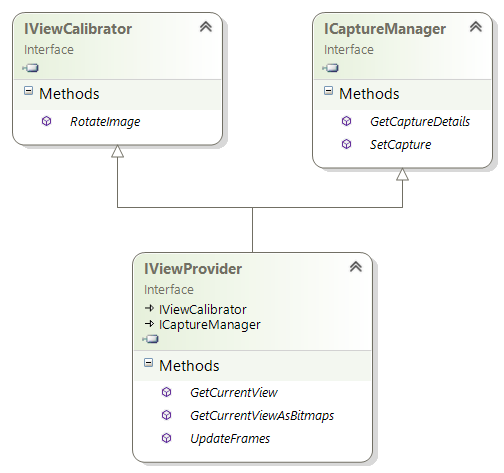
\includegraphics[scale=0.9]{images/IViewProvider}
\caption[Przechwytywanie diagram]{Interfejsy przechwytywania obrazów}
\end{figure}

Interfejs \textit{IViewCalibrator} jest odpowiedzialny za operacje związane z kalibracją obrazu. W~tym projekcie jedyną taką operacją jest obrót obrazu, w celu zrównoważenia ewentualnego obrotu kamery (metoda \textit{RotateImage}).
Interfejs \textit{ICaptureManager} odpowiada za wszystko, co jest związane z przechwytywaniem obrazu. Metoda \textit{SetCapture} ustawia dany kanał na kamerę o danym indeksie w systemie. Indeksy przypisywane są urządzeniom podczas ich wykrywania. Metoda \textit{GetCaptureDetails} pobiera informacje o przechwytywanym obrazie, na przykład rozdzielczość obrazu, jego rotację czy indeks kamery, z której pochodzi.
Interfejs \textit{IViewProvider} jest głównym interfejsem, który jest implementowany przez moduł. Obejmuje sobą funkcjonalności interfejsów poprzednio wymienionych oraz udostępnia metody bezpośrednio związane z pobieraniem obrazu. Metoda \textit{UpdateFrames} wysyła sygnał do wątków pobierających obraz, aby pobrały kolejną klatkę. Pozostałe dwie metody - \textit{GetCurrentView} i \textit{GetCurrentViewAsBitmaps} pobierają obecne klatki w różnych formatach. Pierwsza z nich, wykorzystywana przez proces główny, pobiera obraz jako klasy Image biblioteki EmguCV. Druga jest wykorzystywana przez aplikację konfiguracyjną, a obraz pobrany z jej wykorzystaniem jest postaci klas System.Drawing.Bitmap.

Z powyższego opisu wynika, że najważniejsze operacje modułu to:
\begin{itemize}
\item Wybór kamery dla danego kanału.
\item Pobranie obrazu z wybranych kamer dla obu kanałów
\item Obrót obrazu w celu zrównoważenia ewentualnego obrotu kamery.
\end{itemize}

Poniżej są przedstawione zasady działania każdej z tych operacji:
\begin{description}
\item [Wybór kamery dla danego kanału] \hfill \\
Dla każdego kanału w module jest pole, w którym jest przechowywany obiekt odpowiedzialny za komunikację z daną kamerą. Do tych pól odwołują się pozostałe funkcjonalności, pobierające obraz. W przypadku zmiany kamery w danym kanale, wartość odpowiedniego pola jest podmieniana na obiekt odpowiadający kamerze docelowej. Zmiana ta jest transparentna dla pozostałych funkcjonalności.
\item [Pobranie obrazu z wybranych kamer dla obu kanałów] \hfill \\
Operacja jest zrealizowana wielowątkowo. Każdy z dwóch kanałów ma swój wątek, czeka na sygnał pobrania klatki, pobiera klatkę wykonując jednocześnie jej obrót, wysyła sygnał informujący o zakończeniu pobierania klatki. Operacje te wykonują się w pętli dopóki wątek nie zostanie przerwany.
\item [Obrót obrazu w celu zrównoważenia ewentualnego obrotu kamery] \hfill \\
Moduł przechowuje informację o ilości obrotów o kąt prosty obrazu dla danego kanału. Zwiększenie (zmniejszenie) kąta obrotu polega na inkrementacji (dekrementacji) tej wartości poprzez wywołanie odpowiedniej metody. Na podstawie tej wartości przy pobraniu każdej klatki obliczany jest kąt, o który dany obraz ma być obrócony.
\end{description}

Funkcjonalności modułu są współdzielone przez aplikację główną oraz konfiguracyjną. Ta~część kontraktu, która jest wykorzystywana przez aplikację konfiguracyjną, jest wydzielona jako kontrakt serwisu udostępnionego tej aplikacji, zgodnie ze wzorcem projektowym \textit{fasada}. Dzięki temu ukryte zostały zbędne funkcjonalności modułu z punktu widzenia aplikacji konfiguracyjnej upraszczając jego interfejs.

Podczas testów modułu wystąpiły sytuacje, w których aplikacja zawieszała się na wywołaniu metody z biblioteki EmguCV pobierającej kolejną klatkę z kamery. Występowało to w sytuacji, kiedy obiekt odpowiedzialny za pobieranie obrazu był ustawiony na kamerę, która nie istniała w systemie (jej indeksowi nie odpowiadało żadne urządzenie). Moduł zawiera rozwiązanie zapobiegające tego typu sytuacjom. Przy każdym pobraniu klatki do odpowiedniego pola zapisywany jest czas jej pobrania. Podczas tworzenia instancji modułu tworzony i uruchamiany jest wątek, który co jakiś czas sprawdza czas od ostatniego pobrania klatki dla kanału. Jeżeli jest on większy od ustalonego dopuszczalnego maksimum, to wątek tego kanału jest przerywany, a~w jego miejsce tworzony nowy. 
W zaimplementowanym rozwiązaniu maksymalna dopuszczalna przerwa między klatkami i czas co jaki jest ona sprawdzana wynosi 10 sekund.

\subsection{Moduł przetwarzania obrazu}

Moduł ten odpowiedzialny jest za realizację warstwy pośredniej w  systemie, czyli przetwarzania obrazów po przechwyceniu ich z kamer. Za pojedyncze przekształcenia obrazu odpowiedzialne są klasy implementujące odpowiedni interfejs. Obiekty tych klas zdefiniowane są w kodzie źródłowym aplikacji. Programista korzystający z kontraktu ustalonego przez bibliotekę, może tworzyć własne implementacje klas przetwarzających obraz. Dokładny opis włączania ich w proces przetwarzania, znajduje się w dalszej części rozdziału, opisującej poszczególne elementy biblioteki.

Kluczowym elementem modułu jest sposób włączenia warstwy przetwarzania obrazu w proces przekazywania obrazu od kamery do gogli. Dodatkowo stworzony został kontrakt definiujący metody, które muszą posiadać klasy realizujące operacje przekształceń obrazu.

\pagebreak

\begin{description}

\item [Funkcjonalność przetwarzania obrazu] \hfill \\
\begin{figure}[h]
\centering
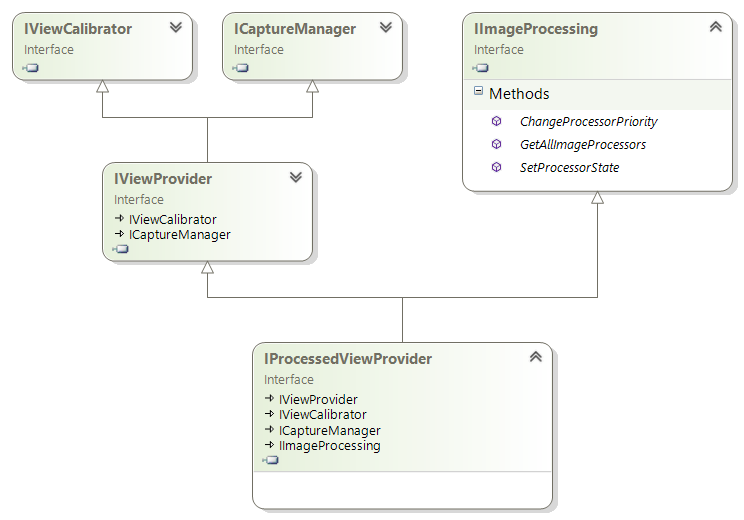
\includegraphics[scale=0.9]{images/IProcessedViewProvider}
\caption[Przetwarzanie diagram]{Interfejsy przetwarzania obrazów}
\end{figure}

Metoda \textit{GetAllImageProcessors} zwraca listę nazw wszystkich dostępnych obiektów przekształcających obraz wraz z informacją o ich aktywności.
Metoda \textit{SetProcessorState} pozwala zmienić stan wskazanego procesora na nieaktywny lub aktywny.
Metoda \textit{ChangeProcessorPriority} pozwala zmienić kolejność wskazanego procesora podczas procesu przetwarzania obrazu. 

Klasą bazową odpowiedzialną za pobieranie obrazu jest \textit{ViewProvider}, implementująca interfejs \textit{IViewProvider}. W celu wprowadzenia nowej warstwy aplikacji odpowiedzialnej za przetwarzanie obrazu, został stworzony interfejs \textit{IProcessedViewProvider} będący rozszerzeniem poprzedniego o dodatkowe metody, związane z zarządzaniem przekształceniami obrazu, które znalazły się w interfejsie \textit{IImageProcessing}. Dodatkowo został zastosowany wzorzec projektowy \textit{Dekorator} poprzez utworzenie nowej klasy \textit{ProcessedViewProvider} implementującej interfejs \textit{IProcessedViewProvider}, będącej rozszerzeniem klasy \textit{ViewProvider} i jej interfejsu, lecz zachowującą część tych samych metod lecz o zmienionym działaniu.

Klasa ta w konstruktorze, jako argument przyjmuje obiekt, implementujący interfejs \textit{IViewProvider}. Kolejnym argumentem przekazywanym w konstruktorze, jest lista obiektów implementujących interfejs \textit{IImageProcessor}. W metodach \textit{GetCurrentView} oraz \textit{GetCurrentViewAsBitmaps} po pobraniu obrazów z pierwotnego obiektu klasy \textit{ViewProvider} wykonywana jest seria przekształceń za pomocą obiektów znajdujących się na wspomnianej liście. W kolejności ich występowania, wywoływana jest metoda \textit{Process} której jako argument przekazywana jest referencja do obiektu reprezentującego obraz. W~ten sposób obrazy zwracane w tych metodach przechodzą przez warstwę przetwarzania obrazów.

\item [Interfejs łączący implementacje przekształceń obrazu] \hfill \\

\begin{figure}[h]
\centering
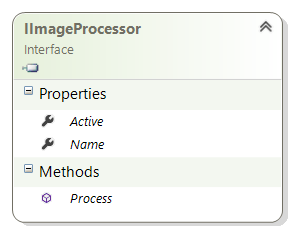
\includegraphics[scale=0.9]{images/IImageProcessor}
\caption[Przekształcenie diagram diagram]{Interfejs obiektu przekształcającego obraz}
\end{figure}

Metoda \textit{Process} jako argument przyjmuje referencje do obrazu reprezentowanego za pomocą typu pochodzącego z biblioteki EmguCV. Operowanie na tym typie pozwala wykorzystać metody pochodzące ze wspomnianej biblioteki, co pozwala na szybszą konwersję obrazu, przeprowadzając część operacji przy wykorzystaniu karty graficznej. Metoda nie zwraca żadnej wartości, lecz operuje na przekazanym obrazie stosując dla niego zaimplementowane przekształcenia.  \\
Dodatkowo interfejs wymaga posiadania przez klasy, następujących właściwości:
\begin{itemize}
\item  \textit{Name}, typu tekstowego - zawierająca nazwę przekształcenia.
\item \textit{Active}, typu logicznego -  decydująca o tym czy przekształcenie będzie wykonane.
\end{itemize}

\end{description}

\subsection{Moduł przekazywania obrazu do gogli}

W tym module znajdują się wszystkie operacje, związane z przekazywaniem przechwyconego obrazu z kamer do gogli. Poprzednie moduły zaimplementowano przy użyciu języka C\# oraz  platformy .NET. Dlatego w celu przekazania obrazu do gogli Oculus Rift, został wykorzystany silnik Unity3D, umożliwiający importowanie zewnętrznych bibliotek, stworzonych w tych technologiach.

Unity3D jest silnikiem grafiki 3D i w podstawowej wersji nie wspiera obsługi urządzeń VR. Jednak producenci gogli zapewniają dedykowane biblioteki programistyczne dla swoich urządzeń, oparte na tym silniku. Pozwalają one na dodanie obsługi wirtualnej rzeczywistosci oraz sterowanie przekazywanym obrazem, dla każdego oka osobno. Wykorzystany został pakiet \textit{Oculus Utitites for Unity} udostępniany przez producenta gogli Oculus Rift (https://developer.oculus.com/downloads/unity/), który w  edytorze silnika Unity funkcjonuje pod nazwą \textit{OVR plugin}.  \hfill \\

\begin{figure}[h]
\centering
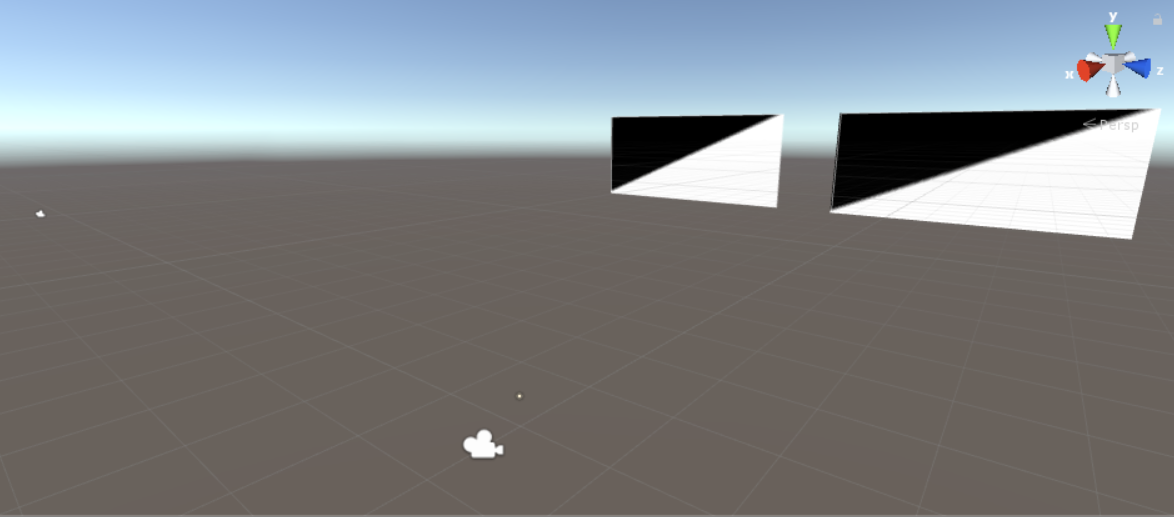
\includegraphics[scale=0.5]{images/unityscene}
\caption[Scena Unity]{Scena w programie Unity Editor}
\end{figure}

Wykorzystując funkcjonalności tego pakietu, stworzona została scena w silniku Unity, zawierająca dwie kamery i dwie tekstury. Kamery posiadają właściwość o nazwie \textit{TargetEye}, która pozwala decydować, czy obraz w polu widzenia kamery trafia do lewego lub prawego ekranu (oka), w urządzeniu Oculus Rift. Na każdej z tekstur również wyświetlany jest obraz tylko dla jednego oka. Tekstury renderowane są jedynie w polu widzenia odpowiedniej kamery, zamiast być wyświetlane jak standardowy obiekt sceny. Dzięki temu podczas obrotów kamery, po wykryciu ruchu urządzenia VR, tekstura nie jest poddawana żadnym przekształceniom, związanym z grafiką 3D, co wpływa na wydajność systemu. W celu wyświetlenia obrazu jako tekstury, potrzebna jest jego odpowiednia konwersja, która jest również ważną częścią modułu.


W module zostały przewidziane następujące interfejsy, zapewniające metody do realizacji kluczowych jego elementów.

\begin{figure}[h]
\centering
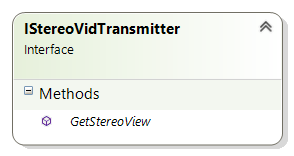
\includegraphics[scale=0.9]{images/IStereoVidTransmitter}
\caption[Przekazywanie diagram]{Interfejs zwracający tekstury do wyświetlenia}
\end{figure}

Interfejs \textit{IStereoVidTransmitter} jest odpowiedzialny za dostarczenie obrazów, w odpowiednim formacie, gotowych do wyświetlenia na scenie programu Unity. Metoda \textit{GetStereoView} zwraca obiekt zawierający dwie tekstury - dla lewego i prawego oka. 

\begin{figure}[h]
\centering
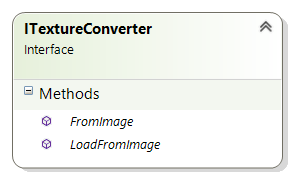
\includegraphics[scale=0.9]{images/ITextureConverter}
\caption[Konwersja diagram]{Interfejs dokonujący konwersji obrazu do tekstury}
\end{figure}

Interfejs \textit{ITextureConverter} odpowiada za wszystkie operacje, potrzebne przy konwersji obrazu do tekstury. W systemie wykorzystywany jest przez klasy implementujące interfejs \textit{IStereoVidTransmitter}. Metoda \textit{FromBitmap} zwraca nowy obiekt tekstury, utworzony na podstawie przekazanego obrazu, za pomocą typu \textit{System.Drawing.Bitmap}. Metoda\textit{FromImage} działa analogicznie do poprzedniej, jednak jako argument przyjmuje obraz reprezentowany za pomocą typu z biblioteki EmguCV.
Metoda \textit{DataFromImage} zwraca tablice typu \textit{byte} z~przekazanego do niej obrazu, która potrzebna jest do konwersji obrazu na teksturę w silniku Unity. Natomiast metoda \textit{LoadFromImage}  ładuje przekazany obraz do wskazanej, istniejącej tekstury. Wykorzystywana jest w celu poprawy wydajności i uniknięcia niepotrzebnego tworzenia tekstur, przy każdej konwersji obrazu.

Z powyższego opisu wynika, że najważniejsze operacje modułu to:
\begin{itemize}
\item Przekazanie i wyświetlanie obrazu
\item Konwersja obrazu
\end{itemize}

Poniżej są przedstawione zasady działania każdej z tych operacji:

\begin{description}
\item [Przekazanie i wyświetlanie obrazu] \hfill \\
Po uruchomieniu aplikacji Unity, wraz ze stworzeniem sceny ładowany jest skrypt działający przez cały czas działania aplikacji. W skrypcie tym inicjowane są klasy odpowiadające za pobieranie obrazu z kamer i poddanie go odpowiednim przekształceniom. Za każdym razem, gdy silnik Unity próbuje odświeżyć obraz, pobierane są dwie klatki obrazu ze wspomnianych klas - dla lewego i prawego oka. Następnie obrazy konwertowane są do postaci tekstury silnika Unity. Po ich przygotowaniu, tekstury na scenie są aktualizowane i do kamer, a później do gogli, trafia odświeżony obraz.
\item [Konwersja obrazu] \hfill \\
Konwersja nie odbywa się w pełni wielowątkowo. Wszystkie operacje na obiektach silnika Unity mogą być realizowane tylko w głównym wątku (dzieje się tak, ponieważ Unity automatycznie wykonuje część operacji na karcie graficznej i ich synchronizacja z wielu wątków jest trudna do zrealizowania). Dlatego obrazy ładowane są do tekstur pojedynczo, co może istotnie spowalniać proces przekazywania ich do gogli.
\end{description}

\subsection{Aplikacja konfiguracyjna}
Moduł ten zrealizowany został w projekcie \textit{ViewVisualization}. W jego ramach została stworzona aplikacja umożliwiająca sterowaniem obrazem trafiającym do gogli.

Do wykonania aplikacji został użyty framework \textit{WPF} (Windows Presentation Foundation). Umożliwia, w wygodny sposób, pogląd obrazu trafiającego do gogli oraz zmianę określonych parametrów sterujących nim. Aplikacja działa jako osobny proces, który komunikuje się z~procesem aplikacji silnika Unity i może działać na innym komputerze. Komunikacja jest możliwa, ponieważ w aplikacji Unity tworzony jest serwis, który umożliwia wywoływanie odpowiednich metod z klasy zajmującej się pobieraniem i przetwarzaniem obrazu (implementacja interfejsu \textit{IViewProvider}). Szczegółowy opis tego serwisu, którego kontrakt został zdefiniowany przy pomocy interfejsu \textit{IViewProviderService} znajduje się w oddzielnym, poświęconym mu rozdziale. Całość aplikacji zrealizowana jest w jednym głównym widoku \textit{MainWindow}, który pojawia się po uruchomieniu aplikacji. 

\begin{figure}[h]
\centering
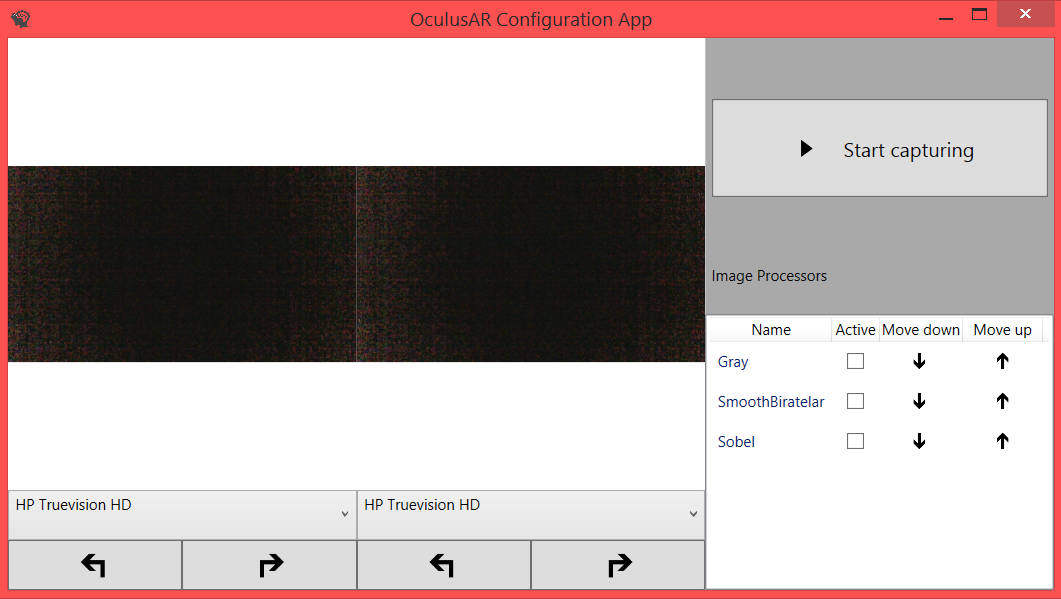
\includegraphics[scale=0.4]{images/mainwindow_screen}
\caption[Widok aplikacji]{Widok aplikacji konfiguracyjnej}
\end{figure}

Widok ten można podzielić na dwie części, ze względu na spełniane funkcjonalności:
\begin{itemize}
\item Wybór źródła i rotacji obrazu
\item Kontrola przetwarzania obrazu
\end{itemize}

W celu większej przejrzystości, dla wymienionych części zostały stworzone specjalne kontrolki \textit{ChannelControl} oraz \textit{SettingsControl}. Każda zawiera interfejs graficzny, który pozwala na realizację określonych dla nich zadań. Jednak, ponieważ został wykorzystany wzorzec \textit{MVVM}, logika zarządzająca nimi znajduje się w klasie \textit{MainViewModel}. 

\begin{description}
\item [Wybór źródła i rotacji obrazu] \hfill \\

Źródło obrazu oraz jego rotacja mogą być ustawione dla każdej kamery osobno, dlatego w aplikacji znajdują się dwie kontrolki \textit{ChannelControl}, zapewniające te funkcjonalności. Każda z nich zawiera następujące elementy:

\begin{itemize}
\item Okno do wyświetlanie obrazu trafiającego go gogli.
\item Lista zawierająca dostępne źródeł obrazu.
\item Przycisk do obrotu obrazu o $90^\circ$ w lewo.
\item Przycisk do obrotu obrazu o $90^\circ$ w prawo.
\end{itemize}

\begin{figure}[H]
\centering
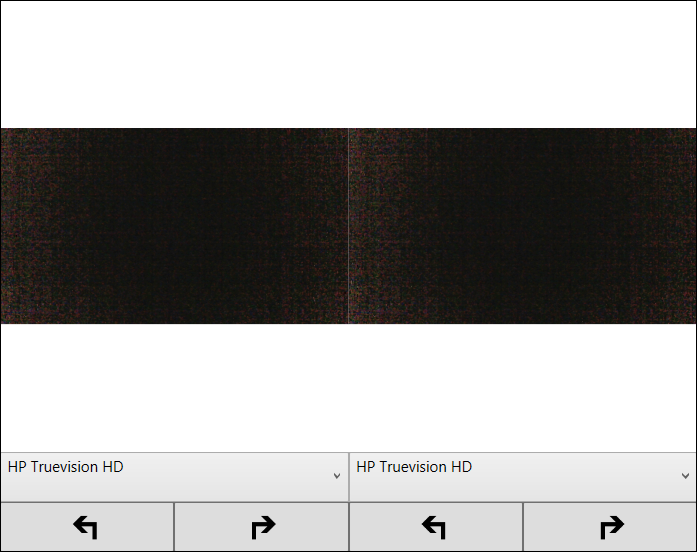
\includegraphics[scale=0.5]{images/channelcontrol_screen}
\caption[Widok aplikacji]{Kontrolki \textit{ChannelControl}.}
\end{figure}

Aplikacja w trakcie działania, za pomoca oddzielnego wątku wywołuje metodę \textit{UpdateFrames} w serwisie {IViewProviderService}, która wywołuje pobranie obrazu z~kamery. Następnie za pomocą metody \textit{GetCurrentViewAsBitmaps} z tego samego serwisu, otrzymuje obrazy z obu kamer w formacie \textit{System.Drawing.Bitmap} i ładuje je do kontrolek wyświetlających obrazy, odświeżając widok całej aplikacji. \\
Zmiana źródła obrazu (kamery) możliwa jest poprzez wybór odpowiedniej opcji z listy, zawierającej wszystkie dostępnymi źródła. Wtedy za pomocą metody \textit{SetCapture} z serwisu, wybierane jest źródło dla lewego lub prawego oka. \\
Obrót obrazu dokonywany jest za pomocą dwóch przycisków. Po kliknięciu jednego z~nich następuje wywołanie metody \textit{RotateImage} z serwisu, która realizuje obrót o $90^\circ$ we wskazaną stronę, dla wybranego oka.

\item [Kontrola przetwarzania obrazu] \hfill \\
Sterowanie przetwarzaniem obrazu jest możliwe, tylko dla obu źródeł obrazu jednocześnie. Dlatego w głównym widoku, umieszczona została jedna kontrolka \textit{SettingsControl}. Zawiera ona listę, na której umieszczone zostały wszystkie dostępne w systemie obiekty do przetwarzania obrazu. Lista dostępnych obiektów pobierana jest z serwisu wystawianego przez aplikację Unity. W celu zarządzania tymi obiektami został stworzony szablon, wyświetlany dla każdej pozycji z listy, składający się z następujących elementów:

\begin{itemize}
\item Nazwa przekształcenia realizowanego przez obiekt.
\item Pole wyboru do aktywowania lub dezaktywowania wybranego przekształcenia.
\item Przycisk do przesunięcia na wcześniejsze miejsce na liście.
\item Przycisk do przesunięcia na kolejne miejsce na liście.
\end{itemize}

\begin{figure}[h]
\centering
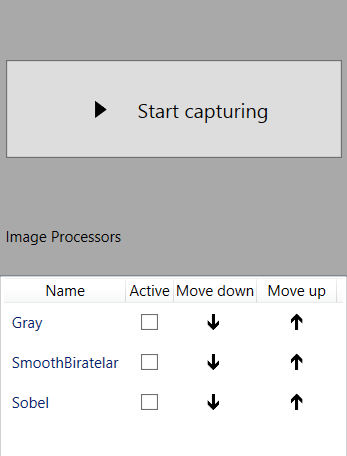
\includegraphics[scale=0.5]{images/settingscontrol_screen}
\caption[Widok aplikacji]{Kontrolka \textit{SettingsControl}.}
\end{figure}

Lista dostępnych przekształceń obrazu wraz z informacją o ich aktywności otrzymywana jest po wywołaniu metody \textit{GetAllImageProcessors} z serwisu \textit{IViewProviderService}. \\
Za pomocą dwóch stanów (zaznaczenie lub brak zaznaczenia)pola wyboru możliwe jest włączanie lub wyłączanie pojedynczych przekształceń. Po zmianie stanu kontrolki wywoływana jest metoda \textit{SetProcessorState}, która ustawia aktywność wybranego obiekty na wskazany stan. \\
Prezentowana lista odpowiada kolejnością liście obiektów przekształcających obraz.  Przekształcenia wykonywane są zaczynając od tego znajdującego się na górze listy. Zarządzanie tą kolejnością możliwe jest za pomocą przycisków, które przesuwają obiekt w~dół lub w górę listy wywołując metodę serwisu o nazwie \textit{ChangeProcessorPriority}.

\end{description}

\subsection{Serwis komunikacji międzyprocesowej}

Ta część systemu odpowiada za komunikację, pomiędzy procesem aplikacji Unity oraz procesem aplikacji konfiguracyjnej. Do tego celu została wykorzystana technologia \textit{WCF}  (Windows Communication Foundation), stworzona przez firmę Microsoft. W założeniu, pierwszą uruchomioną aplikacją powinna być aplikacja Unity, która w momencie startu wystawia serwis w sieci lokalnej pod adresem \textit{http://localhost:{port}/OculusAR}, gdzie port jest wartością pochodzącą z pliku konfiguracyjnego aplikacji. Aplikacja konfiguracyjna podczas uruchomienia próbuje się podłączyć do serwisu znajdującego się pod tym adresem, jeśli wystąpi błąd z połączeniem, użytkownik dostaje stosowny komunikat, informujący o przyczynie błędu. 

Technologia \textit{WCF} wymaga, aby zdefiniować metody będące kontraktem dostępnych operacji, przez klasę, która obsługuje dany serwis. Kontrakt ten zdefiniowany został następująco:
\begin{figure}[h]
\centering
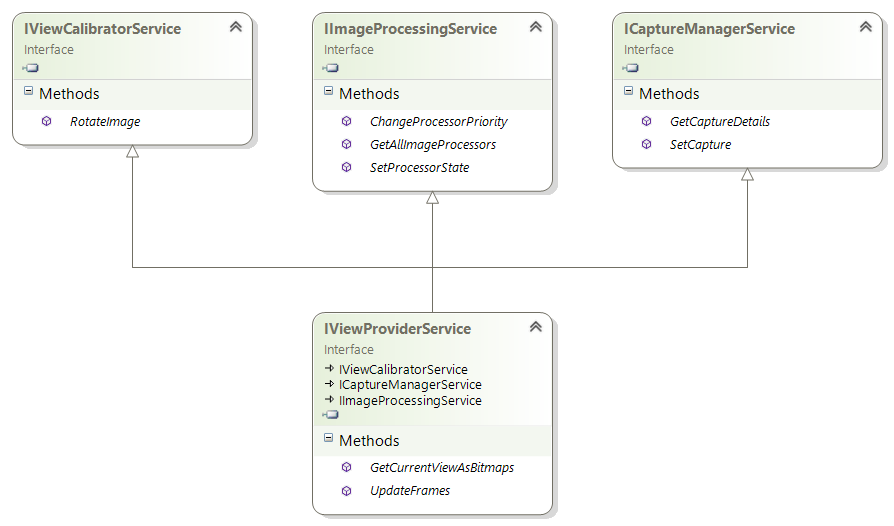
\includegraphics[scale=0.9]{images/IViewProviderService}
\caption[Serwisy diagram]{Interfejsy serwisów}
\end{figure}
 
Opis interfejsów zawartych w kontrakcie:
\begin{itemize}
\item \textit{IViewCalibratorService} - część serwisu odpowiadająca za rotację obrazu.
\item \textit{ICaptureManagerService} - część serwisu odpowiadająca za wybór źródła obrazu dla poszczególnych kanałów.
\item \textit{IImageProcessingService} - część serwisu odpowiadająca za zarządzanie przetwarzaniem obrazu.
tem \textit{IViewProviderService} - serwis składający się ze wcześniej wymienionych części oraz metod związanych z pobieraniem obrazu.
\end{itemize}

Szczegółowy opis metod zawartych w wymienionych interfejsach, został pominięty, ponieważ polegają one na wywołaniu metod o tych samych nazwach z klas implementujących interfejs \textit{IViewProvider}, którego opis znajduje się w poprzedniej części dokumentu.

Interfejs \textit{IViewProviderService} implementowany jest przez następujące klasy:

\begin{itemize}
\item \textit{ViewProviderService}
\item \textit{ViewProviderClient}
\end{itemize}

Pierwsza z nich, odpowiada za utworzenie serwisu pod wspomnianym wcześniej adresem i~wykorzystywana jest przez aplikację Unity, która tworzy serwis w momencie startu.
Natomiast druga klasa jest klientem, który podłącza się do istniejącego serwisu. Metody klienta polegają na wywołaniu metod serwisu o tej samej nazwie. Klasa ta wykorzystywana jest w aplikacji konfiguracyjnej, która za jej pomocą  może sterować procesem pobierania i przetwarzania obrazu, w procesie aplikacji Unity.

 

\chapter{Rezultat pracy}
Ten rozdział jest poświęcony przedstawieniu rezultatów pracy nad omawianym systemem. Omówione zostaną testy, które zostały przeprowadzone w celu zbadania, czy stworzone rozwiązanie odpowiada założeniom, przedstawionym w rozdziale \textit{Cel i założenia projektu}. Rozdział obejmuje także omówienie wniosków wyciągniętych podczas pracy nad tworzonym systemem. 

\section{Konstrukcja gogli}
W celu zapewnienia wrażenia rozszerzonej rzeczywistości niezbędne było zamontowanie kamer na goglach wirtualnej rzeczywistości. Dzięki odpowiedniemu montażowi, uwzględniającemu cechy ludzkiej wizji stereoskopowej uzyskuje się gogle, które wyświetlają użytkownikowi obraz stereoskopowy oraz reagują na ruch głowy, poprzez ruch kamer.
Sposób montażu musiał spełniać dwa wymagania:
\begin{itemize}
\item Niedozwolone są jakiekolwiek stałe modyfikacje gogli.
\item Montaż musi umożliwiać łatwą zmianę odległości między kamerami.
\end{itemize}
W związku z tymi wymaganiami, wykorzystano już zamontowany do gogli uchwyt kontrolera Leap Motion. Kamery zostały przymocowane do uchwytu, składającego się z trzech części:
\begin{itemize}
\item Dwa komponenty, bezpośrednio przymocowane do kamer.
\item Prowadnica, kształtem odpowiadająca kontrolerowi Leap Motion, do której te komponenty zostały przymocowane.
\end{itemize}

\begin{figure}[H]
\centering
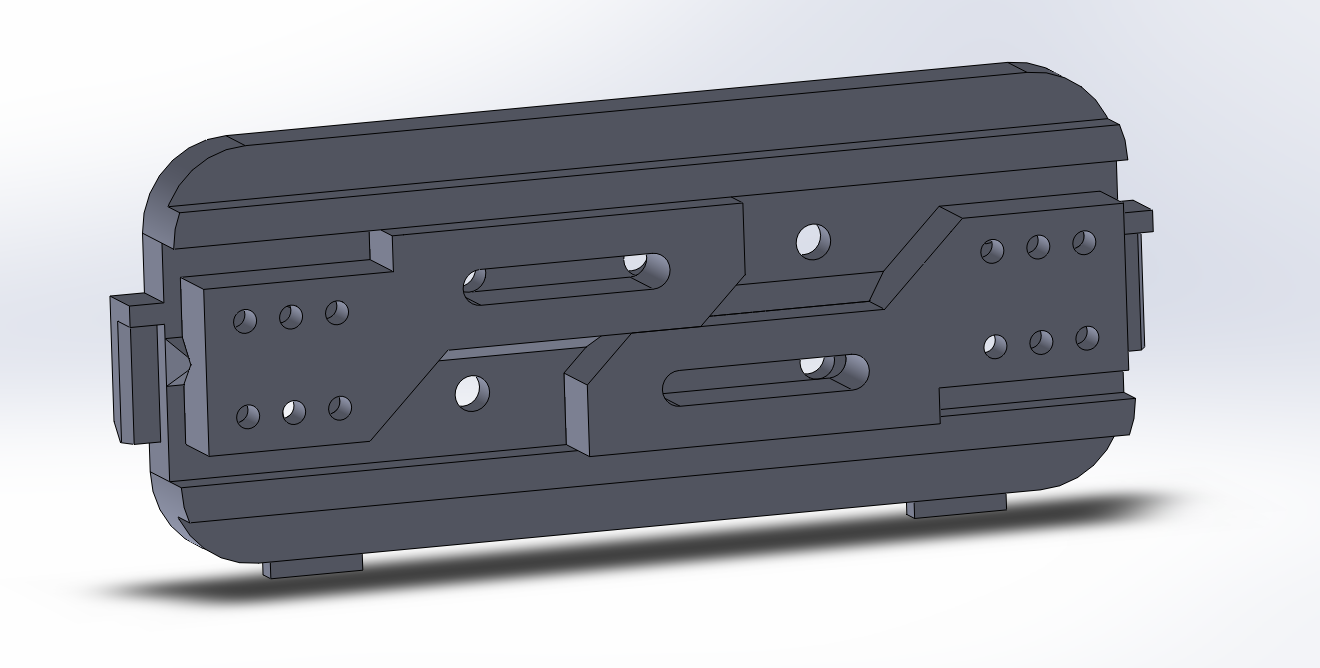
\includegraphics[scale=0.3]{images/cameraHolder}
\caption[Projekt uchwytu]{Projekt uchwytu}
\end{figure}

Części te są połączone ze sobą śrubami. Konstrukcja uchwytu umożliwia przesuwanie kamer po prowadnicy w celu regulacji odległości między kamerami.

Projekt uchwytu wykonał Maciej Spychała - członek Koła Naukowego Wirtualnej Rzeczywistości, absolwent wydziału MiNI.

\begin{figure}[H]
\centering
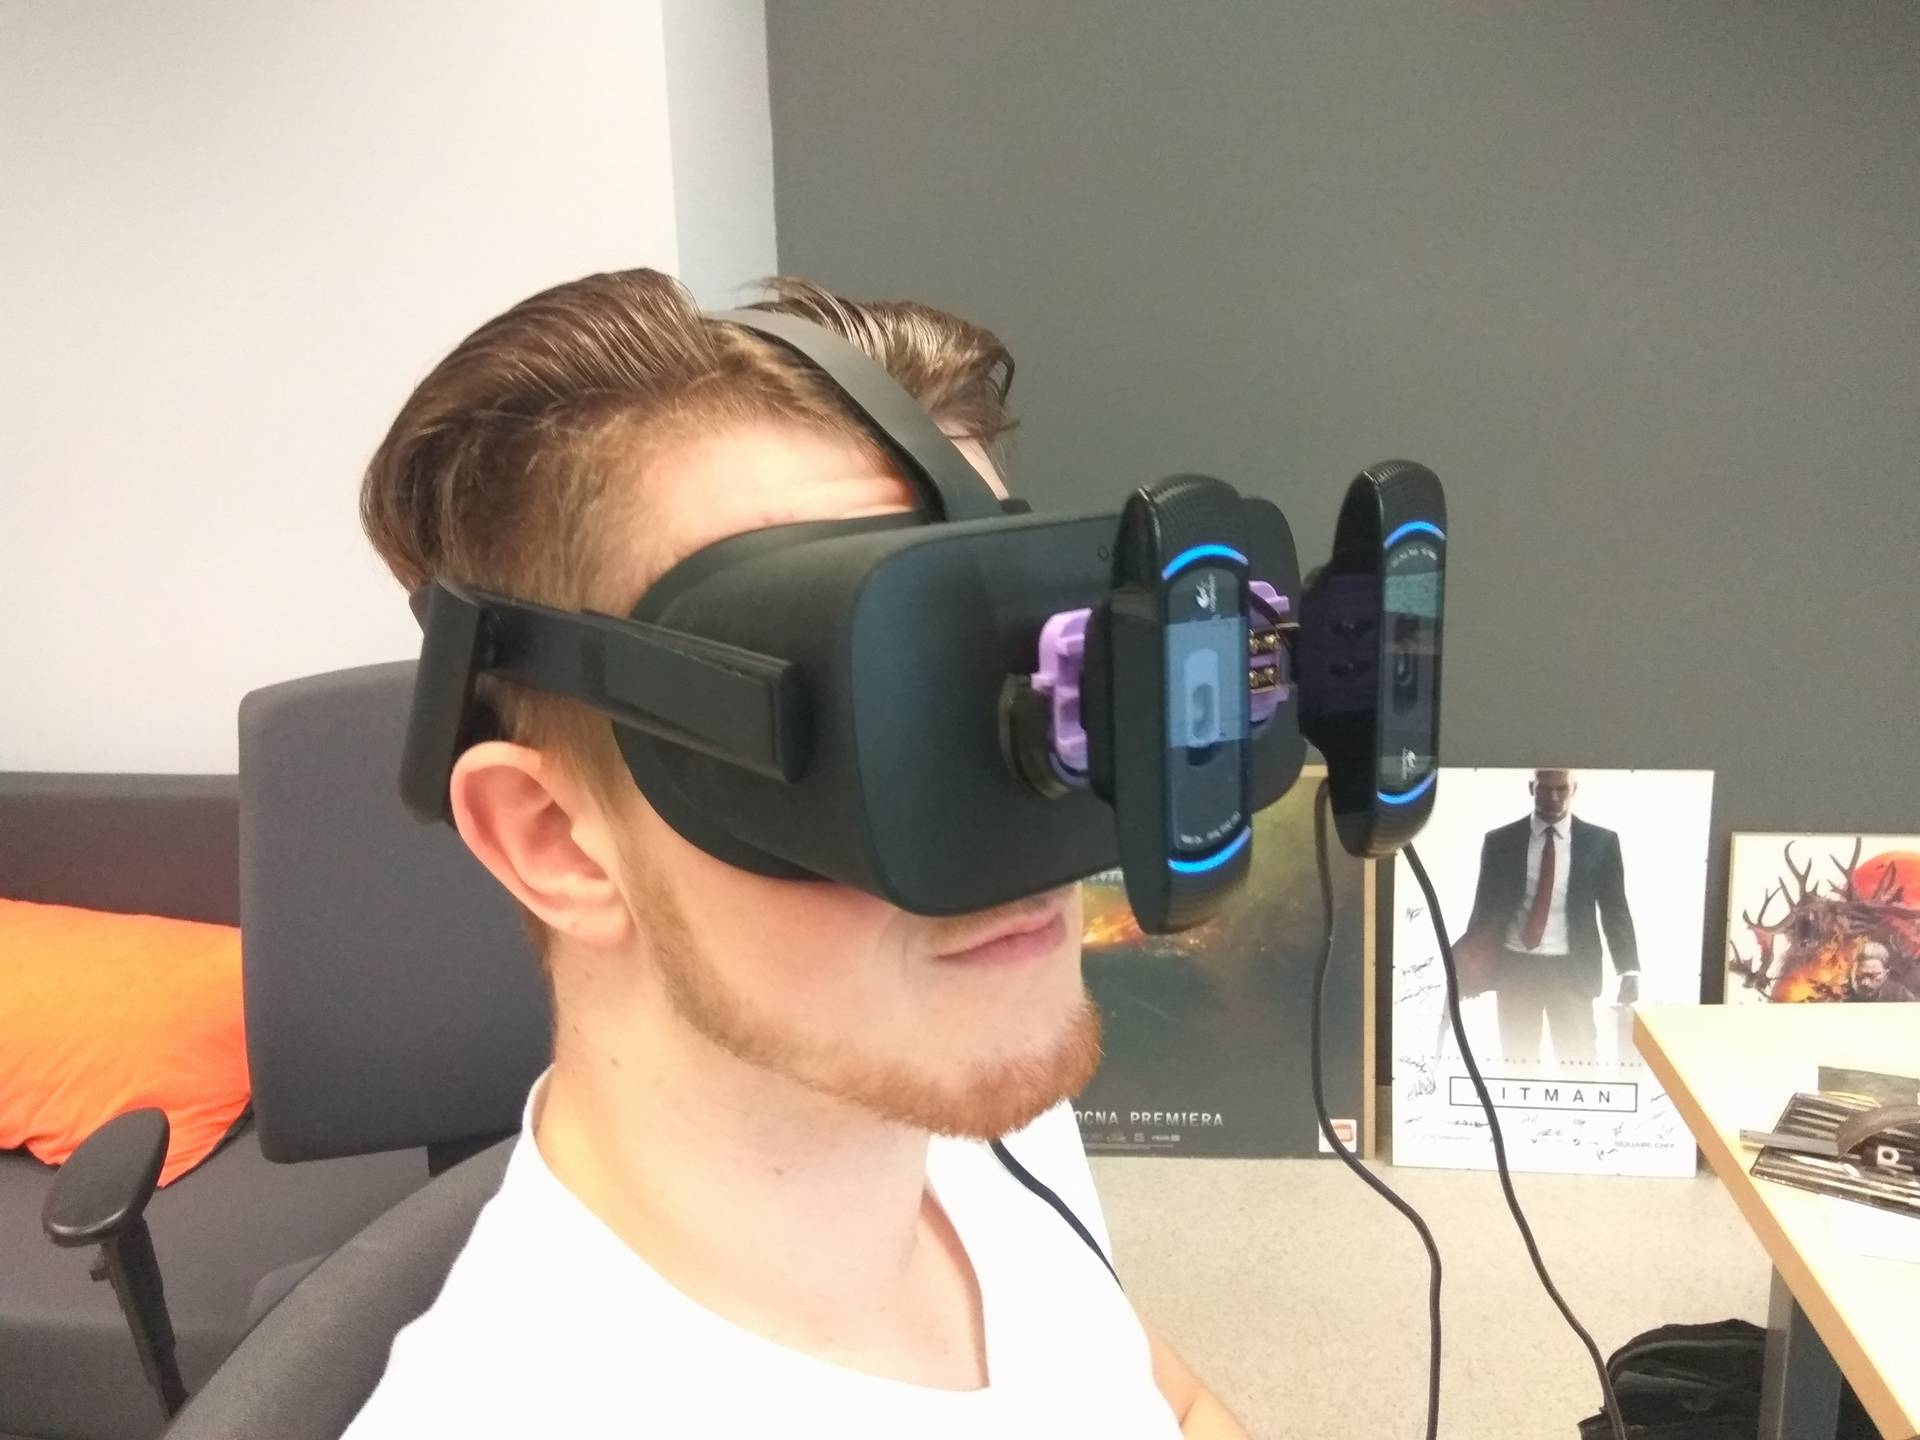
\includegraphics[scale=0.2]{images/googleWithCameras}
\caption[Skonstruowane gogle]{Skonstruowane gogle}
\end{figure}

\section{Testy rozwiązania}
Przeprowadzone testy można podzielić na dwie kategorie. Pierwszą z nich będą testy obiektywne, czyli takie, które można przedstawić w formie danych liczbowych. Tego typu testy będą związane bezpośrednio z wydajnością systemu i jej wpływem na wrażenia użytkownika. Drugą kategorią będą testy subiektywne, opierające się na indywidualnych odczuciach związanych z korzystaniem z kostruowanych gogli AR. 

\subsection{Testy wydajności}
Ten podrozdział jest poświęcony testom wydajności systemu. W związku z tym, że tego typu systemy należą do klasy tzw. systemów czasu rzeczywistego, jest to bardzo istotna kwestia przy tworzeniu takich rozwiązań. Nawet minimalne przekroczenie akceptowalnych przez ludzki organizm opóźnień może bardzo wpłynąć na komfort i ogólne wrażenie z korzystania z gogli.

Wszystkie testy zostały wykonane dla dwóch rozdzielczości obrazu:
\begin{itemize}
\item 1440 x 1080
\item 640 x 480
\end{itemize}

\begin{description}
\item[Opóźnienie przesyłanego obrazu] \hfill \\
Pierwszą z kwestii, która została poruszona jest opóźnienie przesyłania obrazu na linii kamery - gogle. Jest to prawdopodobnie najważniejszy problem, od rozwiązania którego zależy to, czy system będzie nadawał się do użytku. Zbyt duże opóźnienia spowodują, że użytkownik nie będzie w stanie zareagować w odpowiednim czasie na zmiany w otoczeniu, ponieważ informacja o nich dotrze do niego za późno. W ramach testów zmierzono różnicę między czasem wyświetlanej klatki, a czasem rzeczywistym.

\textit{Sposób wykonania testu}

Założenia:
\begin{itemize}
\item Różnicę czasu między wyświetleniem obrazu w aplikacji Unity, a w goglach VR przyjmujemy jako 0 ms. Nie ma możliwości zmiany tego opóźnienia bez ingerencji w kod biblioteki zewnętrznej, zatem nie jest ono objęte w testach.
\item Pomiary wykonywane są przy dwóch podłączonych kamerach. Obie pobierają obraz z taką samą rozdzielczością.
\end{itemize}

Do wykonania testu potrzebne są: kamera, ekran, stoper. Kamera, która będzie wykorzystywana przez aplikację do pobierania obrazu, skierowana jest w stronę ekranu. Stoper należy oprzeć o ekran tak, aby był widziany przez kamerę. Jeżeli wszystko jest ustawione poprawnie, to na ekranie stoper powinien być widoczny dwukrotnie. Widziany bezpośrednio przez kamerę oraz wyświetlany na ekranie. Oba obrazy stopera powinny być na tyle czytelne, aby zatrzymując obraz można było odczytać z niego czas.
Różnica pomiędzy czasem, wyświetlanym na bezpośrednim obrazie stopera, a czasem z jego obrazu ekranowego, jest opóźnieniem danej klatki.
Należy wykonać kilka pomiarów, a następnie na ich podstawie wyznaczyć opóźnienie obrazu.

\textit{Wyniki}

Wykonano po 10 pomiarów opóźnienia obrazu dla każdego z poniższych przypadków:
\begin{itemize}
\item przekazywanie obrazu bez przetwarzania
\item przekazywanie obrazu z konwersją do skali szarości
\item przekazywanie obrazu obróconego o 90\textdegree
\end{itemize}

W poniższej tabeli przedstawione są pomiary:
\begin{table}[H]
\centering
\begin{tabular}{lccc}
Nr & Bez przetwarzania {[}ms{]} & Konwersja do skali szarości {[}ms{]} & Obrót o 90\textdegree {[}ms{]} \\ \hline
1  & 230                        & 220                                  & 290                            \\
2  & 220                        & 200                                  & 190                            \\
3  & 220                        & 220                                  & 260                            \\
4  & 220                        & 190                                  & 230                            \\
5  & 210                        & 260                                  & 280                            \\
6  & 220                        & 230                                  & 260                            \\
7  & 190                        & 160                                  & 300                            \\
8  & 140                        & 240                                  & 220                            \\
9  & 230                        & 210                                  & 220                            \\
10 & 200                        & 180                                  & 270                            
\end{tabular}
\caption{Pomiary opóźnień (rozdzielczość 1440 x 1080)}
\end{table}

\begin{table}[H]
\centering
\begin{tabular}{lccc}
Nr & Bez przetwarzania {[}ms{]} & Konwersja do skali szarości {[}ms{]} & Obrót o 90\textdegree {[}ms{]} \\ \hline
1  & 120                        & 230                                  & 160                            \\
2  & 220                        & 160                                  & 190                            \\
3  & 140                        & 80                                   & 160                            \\
4  & 120                        & 240                                  & 200                            \\
5  & 120                        & 150                                  & 220                            \\
6  & 150                        & 130                                  & 230                            \\
7  & 140                        & 160                                  & 220                            \\
8  & 140                        & 150                                  & 180                            \\
9  & 180                        & 160                                  & 160                            \\
10 & 210                        & 130                                  & 160                            \\ 
\end{tabular}
\caption{Pomiary opóźnień (rozdzielczość 640 x 480)}
\end{table}

Na podstawie powyższych pomiarów wyznaczono średnie opóźnienia dla każdego z tych trzech przypadków oraz dwóch rozdzielczości:

\begin{table}[H]
\centering
\begin{tabular}{r|cc}
                                     & 1440 x 1080 & 640 x 480 \\ \hline
Bez przetwarzania {[}ms{]}           & 208         & 154       \\
Konwersja do skali szarości {[}ms{]} & 211         & 159       \\
Obrót o 90\textdegree {[}ms{]}       & 252         & 188      
\end{tabular}
\caption{Średnie opóźnienia obrazu}
\end{table}


\item[Ilość klatek na sekundę] \hfill \\
Następną kwestią wydajnościową jest ilość klatek na sekundę (FPS). Odpowiednio wysoka ilość FPS jest niezbędna, aby osiągnąć efekt płynności obrazu, na który użytkownik patrzy. Jeżeli ilość ta będzie niewystarczająca osoba, która korzysta z gogli, będzie miała wrażenie zacinania się obrazu. To zjawisko jest zwane potocznie "klatkowaniem".

\textit{Sposób wykonania testu}

Do głównej pętli aplikacji, przetwarzającej klatki, dodano niewielką ilość kodu, który zlicza liczbę iteracji pętli (odświeżeń obrazu) i co ustaloną ilość wypisuje aktualny czas na konsolę. Operacje te nie pobierają dużo mocy obliczeniowej na ich wykonanie zatem można założyć, że ich wpływ na wynik pomiarów jest pomijalny. Dzieląc ustaloną liczbę klatek przez różnicę czasów (w sekundach) wypisanych w dwóch kolejnych iteracjach otrzymano liczbę klatek na sekundę.

\textit{Wyniki}

Wykonano po 10 pomiarów opóźnienia obrazu dla każdego z poniższych przypadków:
\begin{itemize}
\item przekazywanie obrazu bez przetwarzania
\item przekazywanie obrazu z konwersją do skali szarości
\item przekazywanie obrazu obróconego o 90\textdegree
\end{itemize}

W poniższej tabeli przedstawione są pomiary:
\begin{table}[H]
\centering
\begin{tabular}{lccc}
Nr & Bez przetwarzania {[}FPS{]} & Konwersja do skali szarości {[}FPS{]} & Obrót o 90\textdegree {[}FPS{]} \\ \hline
1  & 14,08                       & 14,29                                 & 14,29                           \\
2  & 14,29                       & 14,29                                 & 13,89                           \\
3  & 14,29                       & 14,29                                 & 14,08                           \\
4  & 14,29                       & 14,29                                 & 14,29                           \\
5  & 14,29                       & 14,29                                 & 14,29                           \\
6  & 14,29                       & 14,29                                 & 14,29                           \\
7  & 13,89                       & 14,29                                 & 14,29                           \\
8  & 14,29                       & 14,29                                 & 14,08                           \\
9  & 14,29                       & 14,29                                 & 14,29                           \\
10 & 14,29                       & 14,29                                 & 14,29                           
\end{tabular}
\caption{Pomiary ilości FPS (rozdzielczość 1440 x 1080)}
\end{table}

\begin{table}[H]
\centering
\label{my-label}
\begin{tabular}{lccc}
Nr & Bez przetwarzania {[}FPS{]} & Konwersja do skali szarości {[}FPS{]} & Obrót o 90\textdegree {[}FPS{]} \\ \hline
1  & 18,87                       & 23,81                                 & 24,39                           \\
2  & 23,81                       & 23,26                                 & 21,28                           \\
3  & 23,81                       & 23,81                                 & 24,39                           \\
4  & 23,81                       & 23,26                                 & 23,26                           \\
5  & 23,81                       & 24,39                                 & 23,26                           \\
6  & 23,26                       & 23,81                                 & 23,81                           \\
7  & 23,81                       & 23,81                                 & 23,81                           \\
8  & 23,81                       & 23,81                                 & 23,81                           \\
9  & 24,39                       & 24,39                                 & 23,81                           \\
10 & 23,81                       & 23,81                                 & 24,39                           \\ 
\end{tabular}
\caption{Pomiary ilości FPS (rozdzielczość 640 x 480)}
\end{table}

Na podstawie powyższych pomiarów wyznaczono średnią ilość FPS dla każdego z tych trzech przypadków i dwóch rozdzielczości:

\begin{table}[H]
\centering
\begin{tabular}{r|cc}
\multicolumn{1}{l|}{}                 & 1440 x 1080 & 640 x 480 \\ \hline
Bez przetwarzania {[}FPS{]}           & 14.23       & 23.32     \\
Konwersja do skali szarości {[}FPS{]} & 14.29       & 23.81     \\
Obrót o 90\textdegree {[}FPS{]}       & 14.21       & 23.62    
\end{tabular}
\caption{Średnie ilości FPS}
\end{table}

Z ilości FPS można wyznaczyć ilość milisekund, która jest potrzebna do przetworzenia jednej klatki:

\begin{table}[H]
\centering
\begin{tabular}{r|cc}
\multicolumn{1}{l|}{}                 & 1440 x 1080 & 640 x 480 \\ \hline
Bez przetwarzania {[}ms{]}           & 70.29       & 42.89     \\
Konwersja do skali szarości {[}ms{]} & 70.00       & 41.99     \\
Obrót o 90\textdegree {[}ms{]}       & 70.39       & 42.34
\end{tabular}
\caption{Średnie ilości milisekund na przetworzenie jednej klatki}
\end{table}

\end{description}

Z przeprowadzonych testów wydajnościowych dla rozdzielczości 1440 x 1080 wynika, że czas poświęcony na przetworzenie jednej klatki wynosi około 70 milisekund (wyznaczony na podstawie liczby FPS). Liczba ta znacznie różni się od średniego opóźnienia, które wynosi ponad 200 milisekund. Dla rozdzielczości 640 x 480 różnica jest proporcjonalna. Prawdopodobne przyczyny takiego stanu rzeczy:
\begin{itemize}
\item Opóźnienie kamer
\item Nieoptymalne, wielowątkowe przetwarzanie kilku klatek w tym samym czasie
\end{itemize}

\subsection{Testy użytkowe}

W tym podrozdziale omówione zostaną testy, które zostały wykonane pod kątem zbadania ogólnego wrażenia użytkownika, który korzysta z konstruowanych gogli AR. Podczas testów uwaga była skierowana w stronę uzyskania jak najlepszego odwzorowania naturalnego widzenia ludzkiego. W tym celu sprawdzono czy człowiek, patrząc przez gogle, jest w stanie radzić sobie z czynnościami, które wymagają korzystania ze zmysłu wzroku, a które w normalnych warunkach nie stanowią problemu. Wykonując te testy sprawdzono w jaki sposób wydajność systemu, omówiona w poprzednim podrozdziale, wpływa na koordynację wzrokowo-ruchową człowieka wykorzystującego stworzony system.

\begin{description}
\item[Ogólne wrażenie] \hfill \\
Na początkowym etapie korzystania z gogli użytkownik czuje się dyskomfort, ponieważ efekt zauważalnie odbiega od naturalnego widzenia. Jednak po jakimś czasie organizm się przyzwyczaja i nie zaobserwowano większych negatywnych odczuć, takich jak np. zawroty głowy, których spodziewano się przed rozpoczęciem testów.

Niedogodnością towarzyszącą wszystkim z poniżej wymienionych testów było znaczne przybliżenie obrazu. Wrażenia użytkownika były podobne jak podczas używania lornetki. Spowodowane jest to rozmiarem skonstruowanych gogli, który skutkuje tym, że kamery znajdują się około 12 centymetrów dalej niż oczy użytkownika. Związane z tym jest również ograniczone pole widzenia. Użytkownik nie widzi swojej ręki na wczesnym etapie wykonywanego ruchu. Powoduje to, że użytkownik sięgał w inne miejsca, niż zamierzał i wymagało to korekty, śledząc ruch dłoni wzrokiem. Dodatkowo optyka kamer jest w~wielu aspektach odmienna od optyki ludzkiego oka, co wpływa na uczucie nienaturalnego obrazu.

Wspomniane czynniki powodują istotne problemy z koordynacją wzrokowo-ruchową użytkownika. Czynności wykonywane w normalnych warunkach odruchowo muszą  być uczone od nowa,  powoduje to konieczność większej koncentracji na wykonaniu zadania oraz opóźnienie w jego realizacji.

W przypadku, kiedy kamery będą ustawione w taki sposób, że będą zbiegać do środka nieznacznie bardziej, niż naturalna zbieżność oczu użytkownika, to jest on w stanie skorygować to mięśniami oczu, zwiększając ich zbieżność tak, jakby patrzył na obiekt blisko położony. Umożliwia to uzyskanie efektu widzenia stereoskopowego nawet przy ustawieniu kamer nieznacznie odbiegającym od idealnego, ale jest to dyskomfortowe z powodu męczenia mięśni oczu. W przypadku dłuższego czasu użytkowania jest to niezalecane rozwiązanie.

\item[Czytanie książki] \hfill \\
\textit{Opis} \\
Czytanie książki o standardowym rozmiarze czcionki. \\

\textit{Rezultat} \\
Czytanie tekstu było możliwe, jednak wymagało większego stopnia skupienia, niż bez użycia gogli. Spowodowane jest to gorszą ostrością obrazu, niż w rzeczywistości, co powoduje potrzebę większej koncentracji na rozpoznawaniu liter i śledzenia aktualnie czytanej linii tekstu. Z powodu wspomnianego przybliżenia obrazu, może okazać się, że czytanie książki trzymając ją w rękach na odległości do której użytkownik jest przyzwyczajony, jest niemożliwe. Książka znajduje się w takich przypadkach na niekomfortowej odległości, przez co tekst jest zbyt duży, a ostrość kamer w tym punkcie może nie być wystarczająco dobra. Dlatego najlepsze wrażenie zostało uzyskane oddalając książkę na odległość wyprostowanych rąk lub po umieszczeniu jej na stole i oddaleniu się na odległość, która zapewniała wystarczającą ostrość obrazu.    

\item[Odbijanie piłki do tenisa stołowego] \hfill \\
\textit{Opis} \\
 Za pomocą paletki do tenisa stołowego użytkownik musi podbić piłkę jak największą liczbę razy zanim spadnie ona na ziemię. \\
 
\textit{Rezultat}\\
Użytkownik gogli miał duże problemy z wielokrotnym podbijaniem piłki. Pierwszą niedogodnością była konieczność trzymania paletki na mocno wyciągniętej do przodu ręce. W przypadku próby odbicia piłki znajdującej się blisko ciała,  niemożliwe było odpowiednie szybkie jej zlokalizowanie, ponieważ powiększony i przybliżony obraz powodował zawężone pole widzenia. W przypadku gdy piłka znajdowała się odpowiednio daleko, najlepsze wyniki udało się osiągnąć przy mniejszej częstotliwości odbić, a więc wtedy kiedy lot piłki w powietrzu trwał dłużej. Użytkownik miał wtedy więcej czasu na ustalenie miejsca w którym spadnie piłka i starał się je przewidzieć. Ze względu na opóźnienie obrazu, błyskawiczna reakcja nie była możliwa dlatego, każde odbicie wymagało odpowiedniego wcześniej przewidzenia toru lotu piłki  i przygotowania paletki na jej spadek.  Przy większych częstotliwościach błędy złego ustawienia paletki są mniej kosztowne, jednak wymagają szybszego czasu reakcji, który jest niemożliwy do osiągnięcia ze względu na opóźnienie obrazu. W takich przypadkach, użytkownik odruchowo, zamiast skupiać się na przesyłanym obrazie, próbował odbijać piłkę opierając się na własnym wyczuciu, w~znacznym stopniu ignorując sygnały wzrokowe, które były rozpraszające i niezgodne z~przeczuciami po odebraniu fizycznych bodźców w ręce. 

\item[Gra w łapki] \hfill \\
\textit{Opis} \\
Popularna zabawa, w której największe znaczenie ma czas reakcji. Dwie osoby stają naprzeciwko siebie z wystawionymi dłońmi z przodu tak, aby dłonie jednej osoby były nad dłońmi drugiej. Zadaniem gracza, którego dłonie są niżej, jest uderzenie dłoni drugiego gracza z góry. Drugi gracz broni się poprzez zabranie rąk. Celem testu jest zbadanie jak użytkownik gogli poradzi sobie przeciwko graczowi bez gogli. \\

\textit{Rezultat}\\
Użytkownik gogli nie miał problemu, jeśli jego rolą było uderzenie rąk przeciwnika. Jednak w tym przypadku, opóźnienie obrazu docierającego do oka miało niewielkie znaczenie, ponieważ nie wpływało ono na odruchowo wykonywane uderzenie, które można przeprowadzić równie skutecznie z zamkniętymi oczami. Test wykazał trudności, gdy użytkownik gogli musiał bronić się unikając uderzenia drugiej osoby. Opóźnienie obrazu było na tyle duże, że uniknięcie uderzenia było niemożliwe ponieważ uczucie uderzenie dochodziło do mózgu w podobnym czasie co zauważenie ruchu ręki drugiej osoby.

\item[Chwytanie przedmiotu] \hfill \\
\textit{Opis} \\
Do wykonania testu potrzebne są dwie osoby oraz mały przedmiot, na przykład moneta. Pierwsza z nich, nie korzystająca z gogli, trzyma dłonie na stole. Pod jedną z tych dłoni znajduje się przedmiot. Druga osoba, użytkownik gogli, ma za zadanie jak najszybciej zakryć przedmiot dłonią po tym jak pierwsza go odkryje. Dzięki temu, że użytkownik nie wie, pod którą dłonią znajduje się przedmiot, można zbadać czas jego reakcji i porównać go z czasem, kiedy gogli nie używa. \\

\textit{Rezultat} \\
Podczas tego testu można było zaobserwować dwa czynniki wpływające negatywnie na wynik użytkownika gogli. Pierwszym z czynników było opóźnienie obrazu, które powodowało, że użytkownik zauważał odkrycie przedmiotu po upływie ułamka sekundy. Drugim czynnikiem jest dezorientacja, spowodowana przybliżeniem obrazu, która została wspomniana w ogólnych wnioskach z testów. Powoduje ona, że użytkownik próbując odruchowo jak najszybciej złapać przedmiot, nie trafia w niego przy pierwszej próbie i musi korygować swój ruch w celu złapania przedmiotu. Jeśli użytkownik chciał być dokładny podczas pierwszego ruchu, musiał on wykonać go znacznie wolniej, próbując kontrolować rękę w trakcie jej ruchu. Wymagało to porównania jej pozycji z obrazem docierającym do mózgu. Z tego powodu precyzyjne złapanie przedmiotu jest wykonywane dużo wolniej i~przy większym skupieniu, niż bez założonych gogli.

\item[Celowanie laserem w punkt (statyczny lub dynamiczny)] \hfill \\
\textit{Opis} \\
Za pomocą wskaźnika laserowego użytkownik musi wskazać wyświetlony na ekranie punkt. Ekran znajduje się w znacznej odległości od użytkownika, która pozwala na to aby punkt był dobrze widoczny jednak musi zapewniać stabilną ostrość obrazu.

\textit{Rezultat} \\
Celując w statyczny punkt, użytkownik nie miał problemu z trafieniem go za pomocą wskaźnika. Dobry efekt udało się osiągnąć, ponieważ ruchy ręką ze wskaźnikiem wykonywane są odruchowo. Znaczna odległość od celu powoduje, że zachowana jest wysoka ostrość obrazu. Pierwsze wykonywane ruchy wymagają większej koncentracji i~obserwacji reakcji wskaźnika na ruch ręką, jednak użytkownik bardzo szybko zyskuje świadomość efektu swoich ruchów, przez co jest w stanie bardzo szybko zbliżyć wskaźnik do wyświetlanego punktu, a następnie dokonać tylko drobnej korekty jego położenia, w celu dokładnego trafienia. Gorszy rezultat został osiągnięty podczas testów z dynamicznym, poruszającym się po ekranie punktem. Podobnie jak w pozostałych testach, opóźnienie przesyłu obrazu miało bardzo duże znaczenie. Przy odpowiednio szybko zmieniającym się płynnie położeniu punktu, użytkownik nie był w stanie nadążyć za punktem i jego zmianami kierunku ruchu. Podczas tych prób, trafienie w punkt było rezultatem czysto przypadkowym lub próbą odgadnięcia przez użytkownika gdzie pojawi się punkt w~następnej chwili, jednak śledzenie punktu za pomocą wskaźnika nie było możliwe.

\item[Rzucanie piłką do celu] \hfill \\
\textit{Opis} \\
Do wykonania testu potrzebna jest piłka tenisowa oraz wyznaczony cel. 

\textit{Rezultat} \\
Użytkownik rzucał piłką tenisową, próbując trafić do rąk osoby stojącej na przeciwko niego. W czasie tego testu, najbardziej zauważalna była wada związana z nadmiernym przybliżeniem obrazu. Użytkownikowi wydawało się, że stojąca naprzeciwko osoba znajduje się dużo bliżej niego, niż w rzeczywistości. Dlatego też rzucał piłką ze zbyt małą siła lub zbyt nisko unosząc rękę. Oszacowanie odległości było na tyle mylące, że piłka dotykała ziemi zwykle już w połowie odległości pomiędzy użytkownikiem, a celem.

\end{description}

\section{Wnioski}

Istotnym zagadnieniem dotyczącym wydajności systemu jest konieczność przechwycenia i~przetworzenia obrazu z dwóch, a nie jednej kamery. Wymaga to znacznie większej mocy obliczeniowej oraz rozdzielenia obliczeń między wiele wątków jednocześnie. Silnik grafiki, wykorzystany do przekazywania obrazu do oczu, nie pozwala na równoległe konwersje obrazów trafiających do oczu. Utrudnia to znacznie optymalizację rozwiązania. \\
Wybór technologii wykorzystanych do implementacji projektu działającego w czasie rzeczywistym jest jedną z najważniejszych kwestii, które powinny być bardzo dokładnie przemyślane na etapie projektowania architektury rozwiązania. W stworzonym systemie, wybrane technologie spowodowały duży narzut czasowy na przekazywanie obrazu pomiędzy wszystkimi warstwami. Dodatkowo, nie pozwoliło to na pełną optymalizację systemu, ponieważ użyte biblioteki nie umożliwiają pełnej kontroli nad dokonywanymi operacjami, przez co utrudnione jest wykorzystanie przez programistów np. procesorów graficznych do przyspieszenia obliczeń.

\subsection{Co wyszło dobrze}

Udało się zrealizować zakładaną funkcjonalność systemu. Dzięki wykorzystaniu dwóch kamer, a także odpowiedniemu ich ustawieniu, obraz trafiający do oczu daje pożądany efekt głębi obrazu. Było to jednym z głównych celów niniejszej pracy. Większość istniejących już projektów dotyczących rozszerzonej rzeczywistości wykorzystuje tylko jedną kamerę, dzięki czemu łatwiej jest uzyskać dobrą wydajność i sterować obrazem, ale obraz nie zachowuje głębi właściwej dla rzeczywistego postrzegania przez człowieka. Celem tej pracy było zbadanie możliwości rozszerzonej rzeczywistości w oparciu o widzenie stereoskopowe i udało się to zrealizować. Dodatkowo mając na uwadze dalsze rozwijanie stworzonego systemu, stworzona została warstwa przetwarzania obrazów, która może być rozbudowywana o nowe funkcjonalności. Przygotowane ramy pod tworzenie nowych przekształceń nie narzucają poważnych ograniczeń i mogą posłużyć do stworzenia dowolnych efektów. Została zaimplementowana również komunikacja międzyprocesowa, pomiędzy aplikacją konfiguracyjną, a aplikacją zajmującą się przekazywaniem obrazu. W pierwotnych założeniach projektu nie było wymagania, aby konfiguracja systemu była zrealizowana w postaci osobnego procesu, jednak rozwiązanie to wnosi istotne korzyści do systemu. Proces sterowania parametrami obrazu może odbywać się na innym komputerze, niż jego pobieranie i przekazywanie do gogli.
Uchwyt do kamer, stworzony na potrzeby pracy, zostanie w laboratorium Koła Naukowego Wirtualnej Rzeczywistości, dzięki czemu będzie mógł zostać wykorzystany przy innych tego typu projektach.

\subsection{Co nie wyszło dobrze}

W stworzonym rozwiązaniu nie udało się zapewnić wysokiej wydajności systemu. Wykonywanie prostych manualnych czynności jest utrudnione, ze względu na opóźnienie obrazu. Precyzyjne ruchy ciała w oparciu o bodźce wzrokowe, możliwe są jedynie przy wykonywaniu ich bardzo wolno. U użytkownika występuje odruchowe wspomaganie kontroli ruchów innymi zmysłami niż wzrokowy, w stopniu znacznie większym niż ma to miejsce w~rzeczywistości. Ze względu na techniczne ograniczenia wykorzystywanych gogli, system nie posiada możliwości śledzenia ruchu gałek ocznych. Powoduje to rozbieżności w odczuciach dotyczących obrazu, porównując do rzeczywistego widzenia. Ludzkie oczy poruszają się, dostosowując się do odległości obiektu na który patrzą. W stworzonym rozwiązaniu odtworzenie tej cechy polegałoby na odpowiednim poruszaniu kamer umieszczonych na goglach, jednak poza zakresem niniejszej pracy. Pożądany efekt był osiągany poprzez ręczną korekcję kamer w razie potrzeby. Działanie systemu bywa niestabilne, związane jest to z kilkoma czynnikami. Pośrednio wykorzystywane są sterowniki systemowe dotyczące urządzeń przechwytywania obrazu. Te mogą być różne w zależności od wykorzystywanych kamer lub komputera. Z tego powodu warstwa przechwytywania obrazu może powodować błędy na komputerach innych niż ten, na którym prowadzony był główny proces tworzenia pracy oraz testów z goglami wirtualnej rzeczywistości. Za nieprzewidziane błędy w aplikacji odpowiadają również wykorzystywane biblioteki, będące wciąż w fazie rozwoju i posiadają wewnętrzne błędy, które powodują, czasami niemożliwe do usunięcia, błędy w tworzonym systemie.

\chapter{Przyszłość rozwiązania}

Rozdział poświęcony jest potencjalnym zastosowaniom stworzonego systemu. Porusza także, w jaki sposób można rozszerzyć go o nowe funkcjonalności oraz usprawnić te, które już są w nim zaimplementowane.

\section{Dalszy rozwój systemu}

Przygotowane funkcjonalności systemu umożliwiają wykorzystanie go do prac nad innymi projektami związanymi z tematyką rozszerzonej rzeczywistości. Przygotowane w czasie tej pracy przekształcenia obrazu prezentują jedynie podstawowe możliwości warstwy przetwarzania obrazu. Może być ona wzbogacona, na przykład o przekształcenia wykorzystujące algorytmy sztucznej inteligencji do rozpoznawania obiektów lub osób. Stosowane efekty mogą nie tylko przekształcać obraz za pomocą filtrów, ale także nakładać na niego tekst lub inne informacje, na przykład wskazówki nawigacyjne.

\subsection{Usprawnienia}

Ten podrozdział poświęcony jest usprawnieniom, które można wprowadzić do istniejącego rozwiązania w celu zwiększenia komfortu użytkowania systemu i zwiększenia możliwości wykorzystania go w praktycznych zastosowaniach.

\begin{description}
\item [Zwiększenie wydajności] \hfill \\
Wydajność zaimplementowanego systemu nie jest wystarczająca, aby móc komfortowo korzystać z gogli przez dłuższy czas. Pierwszym krokiem, jaki powinien być podjęty w celu rozwinięcia systemu, powinno być poprawienie procesu przekazywania obrazu z~kamer do gogli. W celu zmaksymalizowania wydajności zalecane jest przepisanie modułu na natywny język programowania, na przykład C/C++. Ponadto warto zwrócić uwagę na sposoby przekazywania obrazu i synchronizacji odpowiedzialnych za to wątków, gdyż prawdopodobnie można je jeszcze zoptymalizować.

\item [Dedykowany układ kamer] \hfill \\
Opisany projekt gogli przewiduje dwie kamery USB podłączone do komputera (lub HUB'u USB). Powoduje to trudności z montażem kamer na goglach, zwiększenie ilości przewodów pomiędzy komputerem, a użytkownikiem oraz konieczność odpowiedniego ustawiania kamer. Proponowanym rozwiązaniem na dalszy rozwój projektu jest stworzenie dedykowanego układu dwóch kamer, zamkniętego w obudowie, umożliwiającego łatwy montaż na goglach VR. Z takiej obudowy można poprowadzić jeden przewód, który obsługiwałby obie kamery. Taki układ zapewniałby odpowiednie ustawienia kamer oraz umożliwiałby wygodną kalibrację kamer, tak jak jest to zrealizowane w przypadku soczewek gogli VR.

\item [Poszerzenie pola widzenia] \hfill \\
Układ gogli i kamer wymusza przesunięcie punktu, w którym obraz jest pobierany, o~pewną odległość do przodu. Różnica odległości między oczami, a kamerą powoduje, że~użytkownik traci z pola widzenia te obszary, które leżą na granicy normalnego wzroku. Ponadto skutkuje to wrażeniem użytkownika, że obiekty, na które patrzy są znacznie bliżej niego niż w rzeczywistości. Aby zastosować tego typu rozwiązanie w praktyce należałoby znaleźć sposób rozwiązania tego problemu, ponieważ, jak wynika to z opisanych testów użytkowych, jest to istotny problem utrudniający wykonywanie podstawowych czynności. Problem wydaje się być ciężki do rozwiązania przy wykorzystaniu obecnie używanych gogli VR i zamontowanych na nich kamer z powodu ich dużych rozmiarów.
\end{description}

\subsection{Dodatkowe funkcjonalności}

Ten podrozdział poświęcony jest pomysłom na dodatkowe funkcjonalności, które zwiększą wartość takiego rozwiązania i umożliwią zastosowanie tworzonej platformy AR w większym zakresie.

\begin{description}
\item [Wykrywanie ruchu gałki ocznej] \hfill \\
W poprzednich rozdziałach poruszono kwestię nienaturalnych wrażeń oraz ograniczeń, związanych z brakiem ruchu kamer umieszczonych na goglach. W celu zniwelowania tego problemu, należy pobierać dodatkowe informacje o ruchu gałek ocznych użytkownika, a~następnie, za pomocą odpowiedniego urządzenia poruszać kamerami według zebranych danych. Takie rozwiązanie pozwoliłoby znacznie poprawić wrażenia z użytkowania systemu oraz ułatwić adaptację mózgu do obrazu, zmieniającego się tak, jak w widzeniu rzeczywistym.

\item [Pobieranie informacji o ruchu głowy] \hfill \\
Przygotowany system wykorzystuje urządzenie, które umożliwia śledzenie ruchu głowy. Dane dotyczące jej położenia nie są jednak wykorzystywane, ponieważ kamery przymocowane są do gogli i obracają się razem z głową. Potencjalnym wykorzystaniem systemu mogą być rozwiązania, w których kamery znajdują się w innym miejscu niż użytkownik oglądający pochodzący z nich obraz. W celu umożliwienia takich zastosowań należałoby dodać możliwość pobrania informacji o obecnym położeniu głowy, a także jej ruchu. Na podstawie zebranych danych można ruch użytkownika odwzorować ruchem urządzenia, na którym są zamontowane kamery. Umożliwiłoby to pobieranie obrazu z~innego miejsca tak, jakby użytkownik się tam znajdował.

\item [Opracowanie szybkiego przesyłu obrazu na odległość] \hfill \\
Funkcjonalnością, która zwiększyłaby potencjał rozwiązania o nowe zastosowania, byłaby możliwość bezprzewodowego połączenia gogli z kamerami. Obecnie wymagane jest aby kamery były podłączone za pomocą kabli do tego samego komputera, co gogle wirtualnej rzeczywistości. Jednak zastosowanie szybkiej transmisji obrazu na odległość, umożliwiłoby wykorzystanie systemu do zdalnego kontrolowania urządzeń w czasie rzeczywistym.

\end{description}

\section{Potencjalne zastosowania}

W tym podrozdziale opisane zostały potencjalne zastosowania, które mogą być celem do osiągnięcia dla tego typu systemów i mogą być motywacją do ich rozwijania. Przedstawione pomysły są dość futurystyczne i mogą wymagać znacznie większej pracy i zaimplementowanych funkcjonalności niż opisane w niniejszej pracy. Nie są do zrealizowania wykorzystując obecnie stworzony system, a wskazują jedynie potencjalny kierunek rozwoju tego typu rozwiązań.

\begin{description}
\item [Zdalnie sterowane roboty] \hfill \\
Takie oczekiwania i wyobrażenia dotyczące wykorzystania rozszerzonej rzeczywistości towarzyszyły jej od samego początku jej rozwoju. Przede wszystkim wojsko mogłoby być zainteresowane stworzeniem robota o sylwetce zbliżonej do człowieka, który byłby kontrolowany zdalnie przez ludzkiego żołnierza. Kamery umieszczone w głowie robota przesyłałyby obraz do człowieka umieszczonego w maszynie przechwytującej ruchy ludzkiego ciała, przekształcając je na ruchy robota. Użytkownik takiej maszyny, przy odpowiednio dobrej głębi obrazu i jego naturalności, mógłby w czasie rzeczywistym reagować na otaczające go wydarzenia. Takie zastosowanie pozwoliłoby połączyć łatwe sterowanie, na wzór ludzkiego, z przewagą fizyczną robota nad ludzkim ciałem. Takie roboty pozwoliłyby też na ograniczenie strat w ludziach, którzy podczas operacji kontrolowaliby roboty z bardziej bezpiecznego miejsca.
  
\item [Zdalne podróżowanie] \hfill \\
Pomimo ogromnego postępu transportu pasażerskiego w ostatnich dekadach, podróżowanie wciąż bywa uciążliwe lub niemożliwe dla wielu osób. Rozwiązaniem takiej sytuacji byłoby umożliwienie zdalnych podróży z przewodnikiem. Użytkownik zakładając gogle wirtualnej rzeczywistości, mógłby wybrać przewodnika z dowolnego rejonu świata, z którym mógłby się połączyć i dołączyć do jego wycieczki. Przewodnik posiadający stację z zamontowanymi kamerami, udostępniałby obraz użytkownikowi oraz mógł opowiadać mu informację na temat miejsca w którym się znajduje. Takie rozwiązanie nie wymaga tworzenia zaawansowanych robotów humanoidalnych, ale udostępnia użytkownikowi zwiedzanie i~poruszanie się po danym obszarze, poprzez głosowe porozumiewanie się z przewodnikiem i ustalanie trasy zwiedzania.
\end{description}
% -------------------- 6. Bibliografia -----------------------
% Bibliografia leksykograficznie wg nazwisk autorów

\begin{thebibliography}{20}%jak ktoś ma więcej książek, to niech wpisze większą liczbę
% \bibitem[numerek]{referencja} Autor, \emph{Tytuł}, Wydawnictwo, rok, strony
% cytowanie: \cite{referencja1, referencja 2,...}

\bibitem[1] {VRdefinition} \emph{Strona internetowa magazynu Komputer Świat},\\http://www.komputerswiat.pl/centrum-wiedzy-konsumenta/gaming/\\wszystko-o-wirtualnej-rzeczywistosci/co-to-jest-wirtualna-rzeczywistosc.aspx

\bibitem[2]{ARMRdifferences} \emph{Strona internetowa firmy Apollogic},\\https://apollogic.com/pl/2017/02/vr-ar-mr-czy-znasz-roznice/

\bibitem[3] {VRdifficulties} \emph{Strona internetowa magazynu Komputer Świat},\\http://www.komputerswiat.pl/centrum-wiedzy-konsumenta/gaming/\\wszystko-o-wirtualnej-rzeczywistosci/niebezpieczenstwa-i-wady-vr.aspx

\bibitem[4]{VRframesPerSecond} \emph{Wypowiedź Vernon Harmon, Technical Account Manager w firmie SCEA, przytoczona w~artykule na stronie TechnoBuffalo},\\https://www.technobuffalo.com/2015/11/20/playstation-vr-framerate-90fps-60fps-minimum/,

\bibitem[5]{VRlatency} \emph{Strona internetowa Tested},\\http://www.tested.com/tech/concepts/452656-challenge-latency-virtual-reality/,

\bibitem[6]{VRsickness} LaViola, J. J. Jr, \emph{A discussion of cybersickness in virtual environments}, ACM SIGCHI Bulletin 32., 2000, 47-56.

\bibitem[7] {IPdistance} \emph{Anthropometric Survey of U.S. Army Pilot Personnel: Methods and Summary Statistics} http://www.dtic.mil/docs/citations/ADA634277, 2012.,

\bibitem[8] {eyeAccomodation} \emph{Strona internetowa HyperPhysics},\\http://hyperphysics.phy-astr.gsu.edu/hbase/vision/accom.html/,

\bibitem[9] {eyeConvergence} Cassin B., Solomon S. \emph{Dictionary of Eye Terminology}, Fl: Triad Publishing Company, 1990,

\bibitem[10] {zbieznosc} \emph{Strona internetowa Światło i Oświetlenie},\\http://www.swiatlo.tak.pl/1/index.php/funkcje-wzroku-akomodacja-adaptacja-zbieznosc/

\end{thebibliography}
\thispagestyle{empty}


% --- 7. Wykaz symboli i skrótów - jeśli nie ma, zakomentować
\chapter*{Wykaz symboli i skrótów}

\begin{tabular}{cl}
HUD & head-up display \\
FPS & frames per second \\
IDE & Integrated Development Environment \\
HTTP & Hypertext Transfer Protocol \\
$\widetilde{}$ & tylda
\end{tabular}
\thispagestyle{empty}


% ----- 8. Spis rysunków - jeśli nie ma, zakomentować --------
\listoffigures
\thispagestyle{empty}


% ------------ 9. Spis tabel - jak wyżej ------------------
\renewcommand{\listtablename}{Spis tabel}
\listoftables
\thispagestyle{empty}



% 10. Spis załączników - jak nie ma załączników, to zakomentować lub usunąć

%\chapter*{Spis załączników}
%\begin{enumerate}[itemsep = 0pt]
%\item Załącznik 1
%\item Załącznik 2
%\end{enumerate}
%\thispagestyle{empty}

% --------------------- 11. Załączniki ---------------------
% to jest po to, żeby było wiadomo, że załączniki znajdują się na końcu pracy

%\newpage
%\pagestyle{empty} 
%Załącznik 1, załącznik 2
\end{document}
